\documentclass[twoside,11pt]{article}

% Use JMLR style with preprint option
\usepackage[preprint]{jmlr2e}
\usepackage{amsmath}
\usepackage{bbm}
% Additional packages (jmlr2e already includes: epsfig, amssymb, natbib, graphicx)
\usepackage{algorithm}
\usepackage{algorithmic}
\usepackage{subcaption}
\usepackage{xcolor}
\usepackage{tikz}
\usetikzlibrary{calc, arrows.meta, decorations.markings, patterns, shapes.geometric, positioning, 3d, decorations.pathmorphing}
\usepackage{array}
\usepackage{tabularx}
\usepackage{listings}
\lstset{basicstyle=\ttfamily, breaklines=true}
\usepackage{booktabs}
\usepackage{xr-hyper}

% Figure search paths (match main paper)
\graphicspath{{./}{./figs/}{../}{attention/}{../../Transformer Manuscript/fig_transformer_validation/}}

% Custom commands (must match main paper)
\newcommand{\softmax}{\operatorname{softmax}}
\newcommand{\KL}{\operatorname{KL}}
\newcommand{\Tr}{\operatorname{Tr}}
\externaldocument[][nocite]{GL(K)_attention}

\begin{document}

\jmlrheading{}{2026}{}{}{}{}{Robert C. Dennis}

\title{Attention as Gauge-Theoretic Variational Inference\\[6pt]
\large Supplementary Material}

\author{\name Robert C. Dennis \email cdenn016@gmail.com \\
  \addr Independent Researcher\\
  \addr Leander, Texas 78641, USA}


\maketitle

\ShortHeadings{Gauge-Theoretic Attention: Supplementary Material}{Dennis}

This supplement collects derivations, implementation details, and additional analyses that support the main paper but are not essential for following the core argument. Appendix~A reviews standard differential geometry for readers from machine learning backgrounds. Appendix~B derives the covariance gradient and its equilibrium analysis. Appendix~C derives the gauge frame gradients for both $\mathrm{SO}(N)$ and $\mathrm{GL}(K)$, including preconditioning strategies. Appendix~D details the numerical methods used for variational gradient descent on the Gaussian and gauge-frame manifolds. Appendix~E records a historical algebraic comparison between BERT dot-product scores and flat-bundle squared-distance scores, together with the limits of its in-sample temperature choice and unavailable current-package inference. Appendix~F develops the renormalization-group universality conjecture and reports synthetic checks of its conditional calculations. Appendix~G retains the theoretical model-channel formalism and identifies the legacy symmetry-breaking simulations as unsupported by the current release. Appendix~H proves the conditional uniqueness of the forward KL divergence via variational duality. Appendix~I derives the prior-bank decode logit from canonical primitives and states the scopes under which the identity is structural rather than dynamical and exact rather than approximate. Appendix~J reports the fixed-$\mathrm{GL}^+(10)$ development-provenance width sweep and identifies the historical divergence-order and positional-prior comparisons as unsupported by the current release.

\appendix

\section{General Mathematical Framework}
\subsection{Principal Bundle and Associated Bundles}

The following geometric and probabilistic constructions comprise standard methods in differential geometry and gauge theory. See references for details, proofs, and examples \citep{nakahara2003geometry,frankel2011geometry,Blei2017,Amari2016}.

Let $\pi: \mathcal{N} \to \mathcal{C}$ be a smooth principal $G$-bundle where $\mathcal{C}$ is a smooth manifold (the base space) and $G$ is a Lie group (the structure group) acting freely and transitively on the right on $\mathcal{N}$. The projection satisfies $\pi(n \cdot g) = \pi(n)$ for all $g \in G$, $n \in \mathcal{N}$.

\paragraph{Bundle triviality.} Throughout the main paper we work with the vertex-frame parameterization $\Omega_{ij} = \exp(\phi_i)\exp(-\phi_j)$, which encodes a \emph{globally trivial} principal $G$-bundle: a single chart $\mathcal{N} \cong \mathcal{C} \times G$ suffices up to gauge equivalence, and the curvature 2-form of the induced connection vanishes identically (Lemma~\ref{thm:vanishing_holonomy} of the main text). The principal-bundle vocabulary developed in this appendix is therefore strictly more general than the parameterization used by the language model and the historical BERT score comparison, both of which live in the flat-bundle subclass. We retain the bundle apparatus because the edge-relaxed extension $\Omega_{ij} = \exp(\phi_i)\exp(\delta_{ij}\cdot G)\exp(-\phi_j)$ equips the bundle with a non-flat discrete connection in which the cocycle condition can fail and a Wilson observable on closed loops is non-trivial; this is the Regime~II discussed in the main text.

Let $\rho_q: G \to \text{Aut}(\mathcal{B}_q)$ and $\rho_p: G \to \text{Aut}(\mathcal{B}_p)$ be representations of $G$ on smooth statistical manifolds $\mathcal{B}_q$ (belief/recognition fiber) and $\mathcal{B}_p$ (model/prior fiber). These fibers are typically $K$-dimensional probability simplices $\Delta^K$ (for categorical distributions) or statistical manifolds with information-geometric structure (e.g., Gaussian manifolds, exponential families).

The associated bundles are:\\
\begin{align}
\mathcal{E}_q &:= \mathcal{N} \times_{\rho_q} \mathcal{B}_q = \left(\mathcal{N} \times \mathcal{B}_q\right)/\sim_q, \\
\mathcal{E}_p &:= \mathcal{N} \times_{\rho_p} \mathcal{B}_p = \left(\mathcal{N} \times \mathcal{B}_p\right)/\sim_p,
\end{align}\\
where $(n \cdot g, b) \sim_u (n, \rho_u(g)b)$ for $u \in \{q,p\}$.

These give fiber bundles $\pi_{\mathcal{E}_q}: \mathcal{E}_q \to \mathcal{C}$ and $\pi_{\mathcal{E}_p}: \mathcal{E}_p \to \mathcal{C}$ with fibers $\mathcal{B}_q(c) \cong \mathcal{B}_q$ and $\mathcal{B}_p(c) \cong \mathcal{B}_p$ at each $c \in \mathcal{C}$.

\subsection{Agents and Multi-Agent Systems}
Agent\\
An agent $\mathcal{A}^i$ is a pair of local sections over a domain $\mathcal{U}_i \subset \mathcal{C}$:

\begin{equation}
\mathcal{A}^i = \left(\sigma^i_q, \sigma^i_p\right),
\end{equation}

where $\sigma^i_q : \mathcal{U}_i \to \mathcal{E}_q$ and $\sigma^i_p : \mathcal{U}_i \to \mathcal{E}_p$.

We write $q_i(c) := \sigma^i_q(c) \in \mathcal{B}_q(c)$ for the belief and $s_i(c) := \sigma^i_p(c) \in \mathcal{B}_p(c)$ for the model at base point $c$. The symbol $p_i$ is reserved in the main paper for the belief-channel base prior $p_i(k_i) \in \mathcal{B}_q$ (a probability density on the belief fiber, see main paper Eq.~\ref{eq:base_priors}); the section $\sigma^i_p$ on the model fiber $\mathcal{B}_p$ defined here is therefore named $s_i$ to avoid collision.

Multi-Agent System\\
A multi-agent system $\mathcal{M}$ over $\mathcal{C}$ is a collection of agents indexed by $\mathcal{I}$:

\begin{equation}
\mathcal{M} = \left\{\mathcal{A}^i = \left(\sigma^i_q, \sigma^i_p\right)\right\}_{i \in \mathcal{I}}.
\end{equation}

Agents generally overlap on intersections $\mathcal{U}_i \cap \mathcal{U}_j$.

Meta-Agent and Epistemic Death\\
A meta-agent is a multi-agent system whose component agents share identical section values on their overlap:

\begin{equation}
q_i(c) = q_j(c), \quad s_i(c) = s_j(c) \quad \text{for } c \in \mathcal{U}_i \cap \mathcal{U}_j.
\end{equation}

A set of agents is epistemically dead if they identically share both beliefs and models. While constituent agents of a meta-agent may be epistemically dead, the meta-agent itself need not be; such agents can be integrated out, yielding coarse-grained higher-order entities and a route toward emergence.

\subsubsection{Hierarchical Meta-Agent Emergence and Cross-Scale Coupling}
\label{sec:appendix_meta_agent}

The gauge-theoretic framework naturally supports the emergence of meta-agents through coarse-graining \citep{kadanoff1966scaling,wilson1974renormalization}. A meta-agent $\mathcal{M}^{(1)}$ is a set of agents $\{i \in I_{\mathcal{M}}\}$ satisfying:

\begin{align}
q_i &= \Omega_{ij} q_j \quad \forall i,j \in I_{\mathcal{M}} \quad \text{(belief consensus)}, \label{eq:belief_consensus} \\
s_i &= \tilde{\Omega}_{ij} s_j \quad \forall i,j \in I_{\mathcal{M}} \quad \text{(model consensus)}. \label{eq:model_consensus}
\end{align}

When these conditions hold, the agents are epistemically dead in that they share identical beliefs and models after accounting for gauge transformations and no longer evolve without continual observations. The meta-agent can be described by a single representative renormalized state $(q_{\mathcal{M}}, s_{\mathcal{M}})$. The cross-scale prior-propagation construction $p_i^{(\zeta)} = \Omega_{i,I}[q_I^{(\zeta+1)}]$ developed in the companion paper \citep{Dennis2025it} treats priors as transported shadows of the meta-agent's posterior at the next-higher scale. The analytic belief-channel reduction in the main paper treats its $p_i$ as primitive boundary data. The retained sweep instead constructs the active same-scale prior through one model-channel refinement, $q_i^{(0)}=p_i=s_i^{(1)}$; this is not the companion paper's cross-scale shadow construction. The hierarchical formulation sketched in this subsubsection is a framework-level scaffold and is not invoked by the retained transformer's single-scale route.

Meta-agents at scale $\zeta=0$ (individual agents) can form meta-agents at scale $\zeta=1$ (groups), which can further coalesce into meta-agents at scale $\zeta=2$ (communities), and so on, creating a hierarchical scale structure:

\begin{figure}[h]
\centering
\small
\[
\text{Agents}^{(0)} \xrightarrow{\text{consensus}}
\text{Meta-agents}^{(1)} \xrightarrow{\text{consensus}}
\text{Meta}^{(2)} \xrightarrow{\text{consensus}} \cdots
\]
\caption{Hierarchical emergence through consensus at successive scales $\zeta$.}
\label{fig:hierarchy}
\end{figure}

At each scale, the effective free energy takes the same form as the full two-channel variational free energy \eqref{eq:free_energy_full_supp}, with agents at scale $\zeta$ replaced by meta-agents at scale $\zeta+1$, coupling constants renormalized according to
\begin{equation*}
  \beta_{ij}^{(\zeta+1)} = f_\beta(\{\beta_{kl}^{(\zeta)}\}), \quad
  \gamma_{ij}^{(\zeta+1)} = f_\gamma(\{\gamma_{kl}^{(\zeta)}\}),
\end{equation*}
and effective gauge frames given by $\phi_{\mathcal{M}}^{(\zeta+1)} = \text{average}(\{\phi_i^{(\zeta)}\})$.
This is the gauge-theoretic analog of renormalization group flow in statistical field theory \citep{anderson1984basic,wilson1974renormalization,garciaperez2018multiscale}. Cross-scale couplings $\Lambda^{\zeta}_{\zeta'}$ mediate interactions between agents at different hierarchical levels via the cross-scale transport operators defined below.

Whether this hierarchical structure maps onto multi-layer transformer architectures (where each layer constitutes a ``scale''), or onto distinct organizational levels within a single attention layer, remains an open question for future investigation.

\subsection{Bundle Morphisms and Transport Operators}
Via standard horizontal lifting from the principal bundle $\mathcal{N}$ to the associated bundles, we obtain a hierarchy of morphisms and induced connections:

Intra-bundle transport operators $\Omega^{(q)}_{ij}: \Gamma(\mathcal{B}_q) \to \Gamma(\mathcal{B}_q)$ (belief-to-belief) and $\Omega^{(p)}_{ij}: \Gamma(\mathcal{B}_p) \to \Gamma(\mathcal{B}_p)$ (model-to-model) act within a single bundle. Cross-scale transport operators $\Lambda^{s}_{s'}: \Gamma^{s}(\mathcal{B}_q) \to \Gamma^{s'}(\mathcal{B}_q)$ (beliefs across scales) and $\tilde{\Lambda}^{s}_{s'}: \Gamma^{s}(\mathcal{B}_p) \to \Gamma^{s'}(\mathcal{B}_p)$ (models across scales) connect different hierarchical levels. Inter-bundle morphisms $\Theta^i_j: \Gamma(\mathcal{B}_q) \to \Gamma(\mathcal{B}_p)$ (belief to model) and $\tilde{\Theta}^i_j: \Gamma(\mathcal{B}_p) \to \Gamma(\mathcal{B}_q)$ (model to belief) relate the two fiber types. Finally, global bundle morphisms $\Phi: \mathcal{E}_p \to \mathcal{E}_q$ (model bundle to belief bundle) and $\tilde{\Phi}: \mathcal{E}_q \to \mathcal{E}_p$ (belief bundle to model bundle) act on the total associated bundles.

Here $\Gamma(\mathcal{B}_u)$ denotes the space of smooth sections over the base $\mathcal{C}$.

\subsection{Gauge Frames and Connections}
Each agent $i$ possesses a local gauge frame field:

\begin{equation}
\phi_i: \mathcal{U}_i \to \mathfrak{g} = \text{Lie}(G),
\end{equation}

which induces a local connection one-form:

\begin{equation}
A^{(i)}_\mu(c) = U_i^{-1}(c) \partial_\mu U_i(c),
\end{equation}

where $U_i(c) = \exp[\phi_i(c)] \in G$. The associated field strength (gauge curvature) is:

\begin{equation}
F^{(i)}_{\mu\nu}(c) = \partial_\mu A^{(i)}_\nu - \partial_\nu A^{(i)}_\mu + [A^{(i)}_\mu, A^{(i)}_\nu] \in \mathfrak{g}.
\end{equation}

When two agents overlap at $c \in \mathcal{U}_i \cap \mathcal{U}_j$, the inter-agent gauge transformation:

\begin{equation}
\Omega_{ij}(c) = \exp[\phi_i(c)] \exp[-\phi_j(c)] \in G
\end{equation}

transports agent $j$'s representations into agent $i$'s frame:

\begin{equation}
q_j(c) \mapsto \Omega_{ij}(c) \cdot q_j(c) := \rho_q(\Omega_{ij}(c))q_j(c).
\end{equation}

On overlaps, local connections are related by:

\begin{equation}
A^{(i)}_\mu = A^{(j)}_\mu + U_j^{-1}\bigl(\Omega_{ij}^{-1} \partial_\mu \Omega_{ij}\bigr) U_j.
\end{equation}

The additive form, rather than the adjoint form $\Omega_{ij} A^{(j)}_\mu \Omega_{ij}^{-1} + (\partial_\mu \Omega_{ij}) \Omega_{ij}^{-1}$, is a consequence of the left-invariant convention $A^{(i)}_\mu = U_i^{-1}\partial_\mu U_i$ together with $\Omega_{ij} = U_i U_j^{-1}$; the familiar adjoint form is recovered under the right-invariant convention $A^{(i)}_\mu = (\partial_\mu U_i) U_i^{-1}$, with the field strength then carrying $-[A_\mu, A_\nu]$.

\paragraph{Scope and forward references.} The present chapter establishes the bundle scaffold and the gauge-connection apparatus used throughout this appendix and the main paper. The remaining foundational machinery on which the main paper's derivations build is developed in subsequent chapters of this appendix: the Gaussian KL closed form under $\mathrm{GL}(K)$ gauge transport and the covariance-channel fixed-point dynamics are derived in Section~\ref{app:covariance_dynamics}; the gauge-frame gradient and the differential of the matrix exponential are derived in Section~\ref{app:phi_gradients}; the natural-gradient descent on the Gaussian manifold and the symmetric positive-definite manifold retraction are derived in Section~\ref{app:variational_descent}. The variational free energy functional itself, its E-step / M-step decomposition, and the softmax-$\beta$ derivation from a mixture-of-sources model are developed in the main paper at Sections~\ref{sec:mixture_derivation} and~\ref{sec:final_free_energy}. The $\mathrm{GL}(K)$-invariance of the Gaussian KL divergence is stated and proved in the main paper at Theorem~\ref{thm:glk_invariance}; this appendix uses it without re-proof.



\section{Covariance Dynamics and Equilibrium Analysis}
\label{app:covariance_dynamics}

\subsection{Covariance Gradient of the Entropy-Suppressed Surrogate}

We derive the own-row covariance derivative for the target-blind entropy-suppressed surrogate. The surrogate omits only the attention-entropy term; it retains the regularized precision sector $\alpha_i^*D_i+R(\alpha_i^*)$. Differentiating through $\beta_{ij}^*=\operatorname{softmax}_j(-E_{ij}/\tau)$ produces the response term $\sum_j(\partial\beta_{ij}^*/\partial\Sigma_i)E_{ij}$. The canonical reduced objective has no such first-order response by the envelope theorem. Neither objective has an adaptive-$\alpha$ response because both retain $R(\alpha_i^*)$.

The own-row surrogate is

\begin{equation}
\mathcal{J}_{\mathrm{surr},i}
=\alpha_i^*D_{\mathrm{KL}}(q_i\|p_i)
+R(\alpha_i^*)
+\sum_{j\in S_i}\beta_{ij}^*D_{\mathrm{KL}}(q_i\|\Omega_{ij}q_j).
\end{equation}

Here $q_i=\mathcal{N}(\mu_i,\Sigma_i)$, $p_i=\mathcal{N}(\mu_{p,i},\Sigma_{p,i})$, and $\sum_{j\in S_i}\beta_{ij}^*=1$.

\subsubsection{Gaussian KL Divergence under $\mathrm{GL}(K)$ Gauge Transport}

The alignment term $D_{\mathrm{KL}}(q_i \| \Omega_{ij} q_j)$ involves KL divergences between Gaussians related by gauge transport $\Omega_{ij} = e^{\phi_i}e^{-\phi_j} \in \mathrm{GL}^+(K)$. The standard Gaussian KL divergence \citep{Bishop2006,murphy2012machine,CoverThomas2006} is

\begin{align}
D_{\mathrm{KL}} \left(
\mathcal{N}(\mu_1, \Sigma_1)
 \|
\mathcal{N}(\mu_2, \Sigma_2)
\right)
&=
\frac{1}{2}
\Big[
\log \frac{|\Sigma_2|}{|\Sigma_1|}
+ \mathrm{tr} \big(\Sigma_2^{-1}\Sigma_1\big)
\\ &\quad
+ (\mu_2 - \mu_1)^\top
  \Sigma_2^{-1}
  (\mu_2 - \mu_1)
- d
\Big].
\label{eq:gaussian_KL}
\end{align}


Differentiating w.r.t.\ $\Sigma_1$ (holding $\mu_1,\mu_2,\Sigma_2$ fixed), using the standard identities $\partial \log|\Sigma|/\partial \Sigma = \Sigma^{-\top}$ and $\partial \mathrm{tr}(A\Sigma)/\partial \Sigma = A^\top$ \citep{petersen2012matrix}, gives

\begin{equation}
\frac{\partial D_{\mathrm{KL}}}{\partial \Sigma_1}
=\frac{1}{2}\left[
-\Sigma_1^{-1}
+ \Sigma_2^{-1}
\right].
\end{equation}

The push-forward $\Omega_{ij} q_j = \mathcal{N}(\Omega_{ij}\mu_j, \Omega_{ij}\Sigma_j\Omega_{ij}^\top)$ used below is the standard linear-transformation rule for a Gaussian random variable under $\Omega \in \mathrm{GL}(K)$ \citep[\S2.3.3]{Bishop2006}. Applying the derivative to the prior and alignment terms gives

\begin{align}
\frac{\partial}{\partial \Sigma_i}
D_{\mathrm{KL}}(q_i \| p_i)
&=\frac{1}{2}\left[
-\Sigma_i^{-1}
+ \Sigma_{p,i}^{-1}
\right],
\\[6pt]
\frac{\partial}{\partial \Sigma_i}
D_{\mathrm{KL}}(q_i \| \Omega_{ij} q_j)
&=
\frac{1}{2}\left[
-\Sigma_i^{-1}
+ (\Omega_{ij}\Sigma_j\Omega_{ij}^\top)^{-1}
\right].
\end{align}

The target-blind inner objective has no observation term. Differentiating the attention-weighted surrogate through the softmax gives

\begin{equation}
\boxed{
\begin{aligned}
\frac{\partial \mathcal{J}_{\mathrm{surr},i}}{\partial \Sigma_i}
&=\frac{1}{2}
\left[
-(1+\alpha_i^*) \Sigma_i^{-1}
+ \alpha_i^*\Sigma_{p,i}^{-1}
+ \sum_{j\in S_i} \beta_{ij}^*
(\Omega_{ij}\Sigma_j\Omega_{ij}^\top)^{-1}
\right] \\
&\quad + \sum_{j\in S_i}
\frac{\partial \beta_{ij}^*}{\partial \Sigma_i}E_{ij}.
\end{aligned}
}
\label{eq:Sigma_gradient_final}
\end{equation}

The first line is the direct derivative shared with the canonical envelope objective. The second line is the surrogate-only response. For two active keys, define $\Delta=E_1-E_2$ and write $E_r'=\partial E_r/\partial\Sigma_i$. The response is exactly

\begin{equation}
-\tau^{-1}\operatorname{Cov}_{\beta}(E,E')
=-\beta_1\beta_2\frac{\Delta}{\tau}(E_1'-E_2').
\label{eq:two_key_near_tie_response}
\end{equation}

For a fixed nonzero gap $|\Delta|=\delta$ and bounded derivatives, its norm is $O(e^{-\delta/\tau}/\tau)$. Along a near-tie path $\Delta=c\tau$, it approaches

\begin{equation}
-\frac{c}{4\cosh^2(c/2)}(E_1'-E_2'),
\label{eq:near_tie_scaled_limit}
\end{equation}

which is generally finite and nonzero rather than $O(\tau)$. At exact equality of the energies the response is zero.

\subsection{Fixed-Point Equation and Symmetric Solution}

For the canonical own-row objective, or for a surrogate configuration in which the response vanishes, setting the direct derivative to zero at $\alpha_i^*=1$ gives

\begin{equation}
\Sigma_i^{-1}
=\frac{1}{2}
\left[
\Sigma_{p,i}^{-1}
+ \sum_{j\in S_i} \beta_{ij}^*
(\Omega_{ij}\Sigma_j\Omega_{ij}^\top)^{-1}
\right].
\label{eq:sigma_fixed_point_beta}
\end{equation}

This is a matrix-valued own-row fixed-point equation. On the entropy-suppressed path, the response in Eq.~\eqref{eq:Sigma_gradient_final} supplies an additional intermediate-temperature term; the canonical first derivative does not contain it.

\subsubsection{Homogeneous limit}

In the homogeneous limit we assume

(i) all agents are identical, so $\Sigma_i = \Sigma_\infty$ for all $i$,

(ii) $\Omega_{ij} \approx I$ (weak misalignment),

(iii) $\Sigma_{p,i} = \Sigma_0$ (shared prior).

Then \eqref{eq:sigma_fixed_point_beta} becomes

\begin{equation}
\Sigma_\infty^{-1}
=\frac{1}{2}
\left[
\Sigma_0^{-1}
+ \Sigma_\infty^{-1}
\right]
\quad\Longrightarrow\quad
\Sigma_\infty = \Sigma_0.
\end{equation}

Hence, in a perfectly symmetric population, the equilibrium covariance reproduces the shared prior.

\subsubsection{Alignment-dominated regime}

Although $\sum_{j\in S_i}\beta_{ij}^*=1$, the concentration of alignment is controlled by $\tau$ in

\begin{equation}
\beta_{ij}^*
=\frac{
\exp \left[
-\frac{1}{\tau}
D_{\mathrm{KL}} \big(q_i \| \Omega_{ij} q_j\big)
\right]
}{\sum_{k\in S_i}
\exp \left[
-\frac{1}{\tau}
D_{\mathrm{KL}} \big(q_i \| \Omega_{ik} q_k\big)
\right]}.
\end{equation}

As $\tau\to0$, $\beta_{ij}^*$ concentrates on the lowest-energy neighbor. Small $\tau$ does not change the coefficient on $\Sigma_i^{-1}$ in Eq.~\eqref{eq:sigma_fixed_point_beta}. A unit coefficient on the alignment term additionally requires $\alpha_i^*\ll1$. In that alignment-dominated regime, the direct fixed point becomes

\begin{equation}
\boxed{
\Sigma_i^{-1}
 \approx 
\sum_{j\in S_i} \beta_{ij}^*
(\Omega_{ij}\Sigma_j\Omega_{ij}^\top)^{-1}
 = \big\langle(\Omega_{ij}\Sigma_j\Omega_{ij}^\top)^{-1}
\big\rangle_{\beta}.}
\label{eq:beta_weighted_precision}
\end{equation}

Here $\langle\cdot\rangle_\beta$ denotes a $\beta^*$-weighted expectation over the active support.

In this regime, agent $i$'s precision matrix becomes the $\beta$-weighted average of transported neighbor precisions. Small $\alpha_i^*$ suppresses the prior term, while small $\tau$ concentrates attention. At $\alpha_i^*=1$, the prior remains at coefficient $1/2$ and Eq.~\eqref{eq:sigma_fixed_point_beta} applies.

When, additionally, all agents already have approximately equal covariances and the transports are near-identity, i.e. $\Sigma_i \approx \Sigma_j$ and $\Omega_{ij} \approx I$, then \eqref{eq:beta_weighted_precision} implies

\begin{equation}
\Sigma_i^{-1} \approx \Sigma_j^{-1}
\quad\Longrightarrow\quad
\Sigma_i \approx \Omega_{ij}\Sigma_j\Omega_{ij}^\top,
\end{equation}

showing that this fixed point is consistent with (rather than deriving) the alignment assumption used in the main text, since the premises $\Sigma_i \approx \Sigma_j$ and $\Omega_{ij} \approx I$ already presuppose near-alignment.

\subsubsection{Gradient flow dynamics}

Let $\mathcal{O}_i$ denote the selected canonical or surrogate own-row objective. Its covariance flow is

\begin{equation}
\frac{d\Sigma_i}{dt}
=-\eta_\Sigma
\frac{\partial \mathcal{O}_i}{\partial \Sigma_i},
\qquad\eta_\Sigma > 0.
\end{equation}

At fixed attention weights $\beta_{ij}$, the equilibrium \eqref{eq:sigma_fixed_point_beta} is a local minimum of the free energy because the $\beta$-fixed Hessian is positive-definite; this establishes $\beta$-fixed convexity, not local attractivity of the full dynamics, which is treated below once the $\beta$-response term is restored. For the Gaussian KL terms $D_{\mathrm{KL}}(\mathcal{N}(\mu_1,\Sigma_1) \| \mathcal{N}(\mu_2,\Sigma_2))$ viewed as a function of $\Sigma_1$ at fixed $\Sigma_2$, the second-variation acts on symmetric tangent vectors $H \in \mathrm{Sym}(K)$ as

\begin{equation}
\left.\frac{\partial^2 D_{\mathrm{KL}}}{\partial \Sigma_1 \partial \Sigma_1}\right[H, H]
=
\tfrac{1}{2} \mathrm{tr}\big(\Sigma_1^{-1} H \Sigma_1^{-1} H\big)
=
\tfrac{1}{2} \big\|\Sigma_1^{-1/2} H \Sigma_1^{-1/2}\big\|_F^2 \geq 0,
\end{equation}

with equality if and only if $H=0$. The Hessian depends only on $\Sigma_1$ and is positive definite for $\Sigma_1\succ0$. The $\beta$-fixed covariance subproblem is therefore strictly convex. This does not prove convexity of the reduced canonical objective: its Hessian contains the negative-semidefinite Schur correction $-\tau^{-1}\operatorname{Cov}_\beta(\partial D_{\mathrm{KL}}/\partial\Sigma_i)$, which can make the reduced Hessian indefinite.

Equation~\eqref{eq:sigma_fixed_point_beta} is the stationarity equation for the $\beta$-fixed covariance subproblem. Row normalization and invertible transport do not by themselves make $\Sigma_i\approx\Omega_{ij}\Sigma_j\Omega_{ij}^\top$ stationary because the prior term remains. That alignment is consistent only in the alignment-dominated regime described above, with $\alpha_i^*\ll1$ and attention concentrated on a nearly aligned neighbor, or when the prior is aligned at the same point. Canonical joint stationarity also requires the entropy-regularized simplex condition. Local attractivity requires the response Schur term to remain dominated by the prior floor, which is not established here.


\section{Gauge Frame Gradients}
\label{app:phi_gradients}

We derive gauge-frame derivatives for both the canonical target-blind objective and its entropy-suppressed surrogate. These derivatives require the differential of the matrix exponential map and differ for compact and general gauge groups.

\subsection{Structure of the Gauge Frame Gradient}

\paragraph{Convention.} Throughout this appendix and Appendix~\ref{app:variational_descent}, the components $\partial \mathcal{F}/\partial \phi_i^a$ of the gauge-frame gradient in the generator basis $\{T_a\}$ are defined via the \emph{right-trivialized} differential of the matrix exponential, $D_{\phi_i}(\exp)[T_a] = Q_a^{R,(i)} \exp(\phi_i)$ with $Q_a^{R,(i)} \equiv \mathrm{dexp}_{\phi_i}(T_a)$, so that $\partial \Omega_{ij}/\partial \phi_i^a = Q_a^{R,(i)} \Omega_{ij}$. The implementation computes these components by automatic differentiation through PyTorch's \texttt{torch.matrix\_exp}, which returns the Fr\'echet derivative $D_\phi(\exp)[T_a]$; the right-trivialized generator is then recovered as $Q_a^R = D_\phi(\exp)[T_a]\cdot e^{-\phi}$. These components may be conditioned by the optional Cartan-modified preconditioner $\tilde g_{ab}$ of Section~\ref{sec:glk_preconditioning} (Eq.~\ref{eq:killing_metric}). The left-trivialized form $\partial/\partial\phi^a \exp(X) = \exp(X)\cdot Q_a^L$ with $Q_a^L = \mathrm{Ad}_{\exp(-\phi)}(Q_a^R)$ is mathematically equivalent and is sometimes written in Appendix~\ref{app:variational_descent} for comparison; the reference implementation uses the right-trivialized convention throughout.

The gauge frames enter through $\Omega_{ij}=\exp(\phi_i)\exp(-\phi_j)$. The global smoothing derivative of the entropy-suppressed surrogate, obtained by differentiating the attention-weighted energies through the softmax, is

\begin{equation}
\frac{\partial \mathcal{J}_{\mathrm{belief,surr}}}{\partial \phi_i}
= \sum_j \left[
\frac{\partial \beta_{ij}}{\partial \phi_i} K_{ij}
+ \beta_{ij} \frac{\partial K_{ij}}{\partial \phi_i}
\right]
+ \sum_k \left[
\beta_{ki} \frac{\partial K_{ki}}{\partial \phi_i}
+ \sum_l \frac{\partial \beta_{kl}}{\partial \phi_i} K_{kl}
\right],
\label{eq:phi_grad_complete}
\end{equation}

where $K_{ij}=D_{\mathrm{KL}}(q_i\|\Omega_{ij}q_j)$. The first sum is the own-row contribution; the second collects key-side contributions from all other rows. The corresponding canonical global smoothing derivative contains only the direct terms,

\begin{equation}
\frac{d\mathcal{F}_{\mathrm{belief,red}}}{d\phi_i}
=\sum_j\beta_{ij}^*\frac{\partial K_{ij}}{\partial\phi_i}
+\sum_k\beta_{ki}^*\frac{\partial K_{ki}}{\partial\phi_i}.
\label{eq:phi_grad_canonical}
\end{equation}

The softmax-response terms in Eq.~\eqref{eq:phi_grad_complete} therefore belong only to the entropy-suppressed surrogate. Independently, filtering retains only the own-row contribution and smoothing retains both sums. Since only $K_{ki}$ depends on $\phi_i$ in row $k$, the surrogate key-side response simplifies to

\begin{equation}
\sum_l \frac{\partial \beta_{kl}}{\partial \phi_i} K_{kl}
= -\frac{\beta_{ki}}{\tau}\frac{\partial K_{ki}}{\partial \phi_i}
\left(K_{ki} - \sum_l \beta_{kl} K_{kl}\right).
\label{eq:reverse_beta_grad_phi}
\end{equation}

This correction vanishes when $K_{ki}$ equals agent $k$'s average divergence $\bar{K}_k = \sum_l \beta_{kl} K_{kl}$, or when $\beta_{ki} \to 0$ (agent $k$ does not attend to $i$).

The coupling weight gradient in the first sum follows from the softmax structure:

\begin{equation}
\frac{\partial \beta_{ij}}{\partial \phi_i} = -\frac{\beta_{ij}}{\tau}\left[
\frac{\partial K_{ij}}{\partial \phi_i} - \sum_k \beta_{ik} \frac{\partial K_{ik}}{\partial \phi_i}
\right].
\label{eq:beta_grad_phi}
\end{equation}

\subsection{Differential of the Matrix Exponential}

All KL gradient terms require the derivative of the transport operator with respect to the gauge frame. For $\Omega_{ij} = \exp(\phi_i)\exp(-\phi_j)$:

\begin{align}
\frac{\partial \Omega_{ij}}{\partial \phi_i} &= \mathrm{dexp}_{\phi_i}(\cdot) \cdot \exp(-\phi_j), \label{eq:dOmega_dphi_i} \\
\frac{\partial \Omega_{ij}}{\partial \phi_j} &= -\exp(\phi_i) \cdot \mathrm{dexp}_{-\phi_j}(\cdot) \cdot \exp(-\phi_j), \label{eq:dOmega_dphi_j}
\end{align}

where $\mathrm{dexp}_\phi: \mathfrak{g} \to \mathfrak{g}$ denotes the differential of the exponential map at $\phi$. For a direction $\xi \in \mathfrak{g}$, the differential is given by \citep{Gallier2020,Hall2015}:

\begin{equation}
\mathrm{dexp}_\phi(\xi) = \sum_{n=0}^{\infty} \frac{1}{(n+1)!} \mathrm{ad}_\phi^n(\xi) = \frac{e^{\mathrm{ad}_\phi} - I}{\mathrm{ad}_\phi}(\xi),
\label{eq:dexp_series}
\end{equation}

where $\mathrm{ad}_\phi(\xi) = [\phi, \xi] = \phi\xi - \xi\phi$ is the adjoint representation. Equation \eqref{eq:dexp_series} defines the right-trivialized differential, related to the Fr\'{e}chet derivative (directional derivative in matrix space) by $D_\phi(\exp)[\xi] = \mathrm{dexp}_\phi(\xi) \cdot e^\phi$. The $\mathrm{GL}(K)$ specialization below uses the Fr\'{e}chet derivative directly via its integral representation~\citep[Ch.~10]{Higham2008}.

\subsubsection{$\mathrm{SO}(N)$ specialization.}

For $\mathrm{SO}(N)$, the gauge frame is expanded in skew-symmetric generators: $\phi = \sum_a \phi^a T_a$ where $T_a \in \mathfrak{so}(N)$, and the gradient is computed component-wise as $\partial \mathcal{F}/\partial \phi^a$. For $\mathrm{SO}(3)$ with $\|\phi\| = \theta$, the differential admits a closed form via the Rodrigues formula:

\begin{equation}
\mathrm{dexp}_\phi(T_a) = T_a + c_1(\theta)[\phi, T_a] + c_2(\theta)[\phi, [\phi, T_a]],
\label{eq:dexp_so3}
\end{equation}

with coefficients:

\begin{equation}
c_1(\theta) = \frac{1 - \cos\theta}{\theta^2}, \qquad c_2(\theta) = \frac{\theta - \sin\theta}{\theta^3}.
\end{equation}

For $\theta < \epsilon$ (numerically $\epsilon \sim 10^{-4}$), Taylor expansions $c_1 \approx \frac{1}{2} - \frac{\theta^2}{24}$ and $c_2 \approx \frac{1}{6} - \frac{\theta^2}{120}$ provide stable evaluation.

\subsubsection{$\mathrm{GL}(K)$ specialization.}

For $\mathrm{GL}(K)$, the gauge frame $\phi \in \mathfrak{gl}(K) \cong \mathbb{R}^{K \times K}$ is a general $K \times K$ matrix. The right-trivialized differential of the exponential does not simplify to a Rodrigues-like formula. The full Fr\'{e}chet derivative $D_\phi(\exp)[\xi] = \mathrm{dexp}_\phi(\xi) \cdot e^\phi$ admits an integral representation \citep[Eq.~10.15]{Higham2008}:

\begin{equation}
D_\phi(\exp)[\xi] = \int_0^1 e^{t\phi} \xi e^{(1-t)\phi} dt,
\label{eq:dexp_integral}
\end{equation}

or equivalently through the $(2K \times 2K)$ block matrix identity \citep[Algorithm~10.27]{Higham2008}:

\begin{equation}
\exp \begin{pmatrix} \phi & \xi \\ 0 & \phi \end{pmatrix}
= \begin{pmatrix} e^\phi & D_\phi(\exp)[\xi] \\ 0 & e^\phi \end{pmatrix}.
\label{eq:dexp_block}
\end{equation}

These give the full Fr\'{e}chet derivative directly; the right-trivialized generator $\mathrm{dexp}_\phi(\xi)$ of Eq.~\eqref{eq:dexp_series} is recovered as $\mathrm{dexp}_\phi(\xi) = D_\phi(\exp)[\xi] \cdot e^{-\phi}$. In practice, automatic differentiation through \texttt{torch.matrix\_exp} provides the $\mathrm{GL}(K)$ differential without explicit computation of \eqref{eq:dexp_integral} or \eqref{eq:dexp_block}.

\subsection{KL Gradient Through Transport}

The KL divergence $K_{ij} = D_{\mathrm{KL}}(q_i \| \Omega_{ij} q_j)$ between $q_i = \mathcal{N}(\mu_i, \Sigma_i)$ and the transported belief $\Omega_{ij} q_j = \mathcal{N}(\Omega_{ij}\mu_j, \Omega_{ij}\Sigma_j\Omega_{ij}^\top)$ depends on $\phi_i$ through $\Omega_{ij}$. Using the Gaussian KL \eqref{eq:gaussian_KL} and the chain rule:

\begin{align}
\frac{\partial K_{ij}}{\partial \phi_i^a}
&= \frac{\partial}{\partial \phi_i^a}\left\{
\frac{1}{2}\left[
\log\frac{|\Omega_{ij}\Sigma_j\Omega_{ij}^\top|}{|\Sigma_i|}
+ \mathrm{tr} \left((\Omega_{ij}\Sigma_j\Omega_{ij}^\top)^{-1}\Sigma_i\right)
+ \Delta\mu_{ij}^\top (\Omega_{ij}\Sigma_j\Omega_{ij}^\top)^{-1} \Delta\mu_{ij}
- K
\right]\right\},
\label{eq:dKL_dphi_expanded}
\end{align}

where $\Delta\mu_{ij} = \mu_i - \Omega_{ij}\mu_j$. Let $\tilde{\Sigma}_{ij} \equiv \Omega_{ij}\Sigma_j\Omega_{ij}^\top$ and $\tilde{\mu}_{ij} \equiv \Omega_{ij}\mu_j$ denote the transported statistics. The derivative has three contributions:

\paragraph{Mean term.} From the Mahalanobis distance:

\begin{equation}
\frac{\partial}{\partial \phi_i^a}\left[(\mu_i - \tilde{\mu}_{ij})^\top \tilde{\Sigma}_{ij}^{-1}(\mu_i - \tilde{\mu}_{ij})\right]
= -2(\mu_i - \tilde{\mu}_{ij})^\top \tilde{\Sigma}_{ij}^{-1} \frac{\partial \tilde{\mu}_{ij}}{\partial \phi_i^a}
- (\mu_i - \tilde{\mu}_{ij})^\top \tilde{\Sigma}_{ij}^{-1} \frac{\partial \tilde{\Sigma}_{ij}}{\partial \phi_i^a} \tilde{\Sigma}_{ij}^{-1} (\mu_i - \tilde{\mu}_{ij}).
\label{eq:mean_term_phi}
\end{equation}

The second term uses the inverse-derivative identity $\partial\tilde{\Sigma}_{ij}^{-1}/\partial\phi_i^a = -\tilde{\Sigma}_{ij}^{-1}(\partial\tilde{\Sigma}_{ij}/\partial\phi_i^a)\tilde{\Sigma}_{ij}^{-1}$, with $\partial\tilde{\Sigma}_{ij}/\partial\phi_i^a$ given by Eq.~\eqref{eq:dtilde_Sigma}; it is generally nonzero and vanishes only where the transported covariance is stationary along $\phi_i^a$.

\paragraph{Trace term.} From the precision-covariance product:

\begin{equation}
\frac{\partial}{\partial \phi_i^a}\mathrm{tr}(\tilde{\Sigma}_{ij}^{-1}\Sigma_i)
= -\mathrm{tr} \left(\tilde{\Sigma}_{ij}^{-1} \frac{\partial \tilde{\Sigma}_{ij}}{\partial \phi_i^a} \tilde{\Sigma}_{ij}^{-1} \Sigma_i\right).
\label{eq:trace_term_phi}
\end{equation}

\paragraph{Log-determinant term.} From the log-determinant ratio:

\begin{equation}
\frac{\partial}{\partial \phi_i^a}\log|\tilde{\Sigma}_{ij}|
= \mathrm{tr} \left(\tilde{\Sigma}_{ij}^{-1} \frac{\partial \tilde{\Sigma}_{ij}}{\partial \phi_i^a}\right).
\label{eq:logdet_term_phi}
\end{equation}

\paragraph{Transport derivatives.} The derivatives of the transported statistics with respect to $\phi_i^a$ are:

\begin{align}
\frac{\partial \tilde{\mu}_{ij}}{\partial \phi_i^a} &= \frac{\partial (\Omega_{ij}\mu_j)}{\partial \phi_i^a}
= Q_a^{(i)} \Omega_{ij} \mu_j, \label{eq:dtilde_mu} \\
\frac{\partial \tilde{\Sigma}_{ij}}{\partial \phi_i^a} &=
Q_a^{(i)} \Omega_{ij} \Sigma_j \Omega_{ij}^\top
+ \Omega_{ij} \Sigma_j \Omega_{ij}^\top (Q_a^{(i)})^\top, \label{eq:dtilde_Sigma}
\end{align}

where $Q_a^{(i)} \equiv \mathrm{dexp}_{\phi_i}(T_a)$ is the right-trivialized differential of the exponential map at $\phi_i$ in the direction of generator $T_a$, defined by the identity $D_{\phi_i}(\exp)[T_a] = Q_a^{(i)} \exp(\phi_i)$. The chain rule applied to $\Omega_{ij} = \exp(\phi_i)\exp(-\phi_j)$ then gives $\partial \Omega_{ij}/\partial \phi_i^a = D_{\phi_i}(\exp)[T_a] \exp(-\phi_j) = Q_a^{(i)} \Omega_{ij}$, which is the form used above. An equivalent expression in terms of the Fréchet derivative is $\partial \Omega_{ij}/\partial \phi_i^a = D_{\phi_i}(\exp)[T_a] \exp(-\phi_j)$. The right-trivialized convention is used consistently when the optional frame preconditioner is evaluated; it does not imply that either outer optimizer routes through a retraction dispatcher.

\subsection{Retraction and Numerical Considerations}

\paragraph{Lie algebra updates.} Since $\phi_i \in \mathfrak{g}$ (a vector space), gradient descent proceeds in the Lie algebra directly:

\begin{equation}
\phi_i \leftarrow \phi_i - \eta_\phi \frac{\partial \mathcal{F}}{\partial \phi_i},
\label{eq:phi_update}
\end{equation}

where $\eta_\phi$ is the gauge frame learning rate. The basic update applies no metric correction (Fisher-Rao or otherwise): the exponential map $\exp: \mathfrak{g} \to G$ provides coordinates for the Lie group, and the gradient lives in $\mathfrak{g}$. The optional gauge-aware preconditioners of Section~\ref{sec:glk_preconditioning} below condition the non-compact directions. In the audited sweep, $\texttt{e\_phi\_lr}=0$ freezes $\phi$ within the E-step, while the unrolled outer cross-entropy graph trains the token-frame table. At each recorded source SHA, the committed optimizer gate combined with $\texttt{m\_phi\_natural\_grad=false}$ routes that table to plain AdamW at learning rate $0.015$ and weight decay $0.05$. Because every run has a provenance record with $\texttt{git\_dirty=true}$ and no dirty diff survives, the exact executed optimizer implementation cannot be independently reconstructed. The heavy-ball field belongs only to the disabled custom outer optimizer; the pullback field can serve either optional frame route but is inactive here because both routes are off.

\paragraph{$\mathrm{SO}(N)$ retraction.} For compact groups such as $\mathrm{SO}(N)$, the optional in-E-step frame-revision route calls \texttt{retract\_son} (the skew-symmetric branch of \texttt{retract\_phi}): the tangent step $\eta_\phi^E\delta\phi$ is clamped to a coordinate trust region (default $0.3$), composed through the order-4 Baker-Campbell-Hausdorff product, and radially rescaled at $\mathrm{max\_norm}=\pi$. This E-step dispatcher is gated off when $\texttt{e\_phi\_lr}=0$, as in every audited sweep configuration. Neither plain AdamW nor the optional custom outer frame optimizer calls it.

\paragraph{$\mathrm{GL}(K)$ updates.} For $\mathrm{GL}(K)$, a single matrix exponential $\exp: \mathfrak{gl}(K) \to \mathrm{GL}^+(K)$ is not surjective onto the identity component \citep{culver1966existence}, but the pairwise transport $\Omega_{ij} = \exp(\phi_i)\exp(-\phi_j)$ covers all of $\mathrm{GL}^+(K)$ via polar decomposition \citep[\S8]{Higham2008}: for any $A \in \mathrm{GL}^+(K)$ with polar decomposition $A = UP$ ($U \in \mathrm{SO}(K)$, $P \in \mathrm{Sym}_{++}(K)$), the exponential map restricts to a surjection $\mathfrak{so}(K) \twoheadrightarrow \mathrm{SO}(K)$ on the compact factor and a bijection $\mathrm{Sym}(K) \xrightarrow{\sim} \mathrm{Sym}_{++}(K)$ on the symmetric factor, so choosing $\phi_i \in \mathfrak{so}(K)$ with $\exp(\phi_i) = U$ and $\phi_j \in \mathrm{Sym}(K)$ with $\exp(-\phi_j) = P$ realizes $A$. This is a per-edge existence statement, not simultaneous graphwise freedom: shared vertex frames force $\Omega_{ij}\Omega_{jk}=\Omega_{ik}$. Because $\phi_i$ lies in the vector space $\mathfrak{gl}(K)$, outer optimizers take additive coordinate steps. The group-aware \texttt{retract\_phi} dispatcher belongs only to optional in-E-step frame revision and is gated off by $\texttt{e\_phi\_lr}=0$ in the audited sweep. The separate custom outer frame optimizer, enabled only by $\texttt{m\_phi\_natural\_grad=true}$, may precondition its gradient but also takes a direct additive coordinate step; it does not call the dispatcher. Plain AdamW likewise updates frame coordinates additively.

\subsection{Gauge Frame Preconditioning for $\mathrm{GL}(K)$}
\label{sec:glk_preconditioning}

While the basic update~\eqref{eq:phi_update} uses the Euclidean gradient in the Lie algebra, the non-compact structure of $\mathrm{GL}(K)$ introduces a numerical asymmetry that motivates gauge-aware preconditioning. The Lie algebra decomposes via the Cartan involution $\theta(X) = -X^\top$ as:

\begin{equation}
\mathfrak{gl}(K) = \underbrace{\mathfrak{so}(K)}_{\text{compact (skew-symmetric)}} \oplus \underbrace{\mathrm{Sym}_0(K)}_{\text{non-compact (traceless symmetric)}} \oplus \underbrace{\mathbb{R}}_{\text{center (trace)}},
\label{eq:cartan_decomposition}
\end{equation}

where $\mathfrak{so}(K) = \{X : X + X^\top = 0\}$ generates rotations and $\mathrm{Sym}_0(K) = \{X : X = X^\top, \operatorname{tr} X = 0\}$ is the traceless symmetric space generating volume-preserving shears (we reserve $\mathrm{Sym}(K)$ for all symmetric matrices, so that $\mathrm{Sym}(K) = \mathrm{Sym}_0(K) \oplus \mathbb{R}\cdot I$). The right-trivialized factor $\Psi(\operatorname{ad}_\phi)$ distinguishes compact and noncompact adjoint directions: on compact rotations its norm remains bounded away from adjoint resonances, while noncompact adjoint eigenvalue gaps can yield exponential amplification. This statement concerns $\Psi(\operatorname{ad}_\phi)$, not the full Fr\'echet derivative $D_\phi\exp[T]=\Psi(\operatorname{ad}_\phi)(T)\exp(\phi)$. Even when $T$ commutes with $\phi$, the $\Psi$ factor equals the identity but the right factor can grow; for example, $\phi=tI$ gives $D_\phi\exp[T]=e^tT$. The optional preconditioners below address coordinate conditioning without supplying a full-$\mathrm{GL}(K)$ invariant metric.

We describe four conditioning strategies. Three are available in the reference code: norm clipping (1), the regularized Cartan-involution-modified Killing-form construction (3), and the exponential-coordinate Frobenius pullback (4). A block-diagonal \texttt{killing\_per\_block} variant of (3) is also available; the Cartan-dampening projector (2) is derived below but is not wired into the released training path. These modes were inactive in the audited sweep because both the optional in-E-step frame update and the custom outer frame optimizer were disabled.

\paragraph{1. Norm clipping (baseline).}
Simple gradient norm clipping $\tilde{g} = g \cdot \min(1, c/\|g\|)$ with threshold $c$. No geometric awareness; treats all Lie algebra directions uniformly.

\paragraph{2. Cartan preconditioning.}
Decompose the gradient into compact and non-compact components and selectively dampen the latter. Given Lie algebra generators $\{T_a\}_{a=1}^{n_{\mathrm{gen}}}$ with Gram matrix $G_{ab} = \operatorname{tr}(T_a^\top T_b)$ and symmetric inner product $S_{ab} = \operatorname{tr}(T_a T_b)$, the projector onto the symmetric subspace is:

\begin{equation}
P_{\mathrm{sym}} = \tfrac{1}{2}G^{-1}(G + S),
\end{equation}

and the preconditioner is $M = I - (1 - \lambda_{\mathrm{sym}}) P_{\mathrm{sym}}$ with dampening factor $\lambda_{\mathrm{sym}} \in (0, 1)$ (typically $0.1$, corresponding to $10\times$ dampening of symmetric directions). The preconditioned gradient is $\tilde{\nabla}_\phi \mathcal{F} = M \cdot \nabla_\phi \mathcal{F}$. Here $P_{\mathrm{sym}}$ acts as $X \mapsto \tfrac{1}{2}(X + X^\top)$ and so retains the trace/dilation direction ($P_{\mathrm{sym}}(I) = I$): it projects onto the full symmetric subspace $\mathrm{Sym}_0(K) \oplus \mathbb{R}\cdot I$ and damps the shear and dilation directions together, rather than the traceless $\mathrm{Sym}_0(K)$ of Eq.~\eqref{eq:cartan_decomposition} alone.

\paragraph{3. Cartan-involution-modified bilinear form (compact-form metric).}
The Killing form of $\mathfrak{gl}(K)$ is $B(X, Y) = 2K \operatorname{tr}(XY) - 2\operatorname{tr}(X)\operatorname{tr}(Y)$. On the trace-free subalgebra $\mathfrak{sl}(K) = \ker(\operatorname{tr})$ it reduces to $B|_{\mathfrak{sl}(K)}(X,Y) = 2K\operatorname{tr}(XY)$, and on the center $\mathbb{R}\cdot I$ it vanishes identically. The Killing form is \emph{indefinite} on real $\mathfrak{sl}(K)$ for $K\geq 2$: under the Cartan decomposition $\mathfrak{sl}(K) = \mathfrak{so}(K) \oplus \mathrm{Sym}_0(K)$ (skew $\oplus$ traceless-symmetric), $B$ is \emph{negative} on $\mathfrak{so}(K)$ and \emph{positive} on $\mathrm{Sym}_0(K)$~\citep{Hall2015,Gallier2020}.

The optional constant construction is not the Killing form itself but the Cartan-involution-modified bilinear form $g(X, Y) = -B(X, \theta(Y))$ with $\theta(X) = -X^\top$ \citep[Ch.~VI]{Knapp2002}. Equivalently, in the generator basis:

\begin{equation}
\tilde{g}_{ab} = 2K \operatorname{tr}(T_a^\top T_b) - 2\operatorname{tr}(T_a)\operatorname{tr}(T_b),
\label{eq:killing_metric}
\end{equation}

which is positive definite on $\mathfrak{sl}(K)$ (the transpose flips the sign on $\mathfrak{so}(K)$, since $\operatorname{tr}(T_a^\top T_a) = -\operatorname{tr}(T_a^2) = \|T_a\|_F^2 > 0$ for skew $T_a$) and degenerate on the center $\mathbb{R} \cdot I$. The implemented regularization $\tilde{g} \mapsto \tilde{g} + \epsilon I$ makes the coordinate matrix positive definite. This compact-form construction agrees with $-B$ up to scale on $\mathrm{SO}(K)$ and assigns positive lengths to both rotations and shears. The Frobenius pairing $\operatorname{tr}(X^\top Y)$ satisfies $\operatorname{tr}((gXg^{-1})^\top(gYg^{-1})) = \operatorname{tr}(X^\top Y)$ for all $X,Y$ when $g^\top g$ is a scalar multiple of the identity. It is therefore invariant under the conformal-orthogonal subgroup $\mathbb{R}^{\times}\mathrm{O}(K)$, whose central scalar factor acts trivially under $\mathrm{Ad}$, but not under a general $\mathrm{GL}(K)$ element. Consequently, $\tilde{g}^{-1}\nabla_\phi\mathcal{F}$ is an $\mathrm{O}(K)$-invariant, more precisely conformal-orthogonal-$\mathrm{Ad}$-invariant, Lie-algebraic preconditioned direction, not a full-$\mathrm{GL}(K)$-covariant natural gradient. A connected Lie group admits a positive-definite bi-invariant metric only when $\mathrm{Ad}(G)$ has compact closure~\citep{Milnor1976}, which fails for noncompact $\mathrm{GL}(K)$.

\paragraph{4. Exponential-coordinate Frobenius pullback (extrinsic and position-dependent).}
This optional construction pulls the Frobenius inner product on $\mathrm{Mat}(K)$ back through the exponential map. The Fréchet derivative of $\exp$ at $\phi \in \mathfrak{g}$ in direction $T_a$ admits the right-trivialized form \citep[\S2.7 / Theorem 5.4]{Hall2015}:

\begin{equation}
D_\phi(\exp)[T_a] = \Psi(\mathrm{ad}_\phi)(T_a) \cdot \exp(\phi), \qquad \Psi(z) = \frac{e^z - 1}{z} = \sum_{k=0}^{\infty} \frac{z^k}{(k+1)!},
\end{equation}

where $\mathrm{ad}_\phi(X) = [\phi, X]$ is the adjoint action and $\Psi(z) = (e^z - 1)/z$ is the generating series for the right-trivialized differential; its multiplicative inverse $z/(e^z-1)$ is the Bernoulli generating function whose Taylor coefficients are the Bernoulli numbers and which appears in $d\exp^{-1}$ and the Magnus expansion~\citep{Hall2015}. The equivalent left-trivialized form is $D_\phi(\exp)[T_a] = \exp(\phi) \cdot ((I - e^{-\mathrm{ad}_\phi})/\mathrm{ad}_\phi)(T_a)$, related by the operator identity $\Psi_R(z) = e^z \Psi_L(z)$. The Frobenius pullback metric on $\mathfrak{g}$ is then:

\begin{equation}
\mathcal{G}_{ab}(\phi)
=\langle D_\phi(\exp)[T_a], D_\phi(\exp)[T_b]\rangle_F
= \operatorname{tr}\bigl(\Psi(\mathrm{ad}_\phi)(T_a)^\top \Psi(\mathrm{ad}_\phi)(T_b) \cdot \exp(\phi)\exp(\phi)^\top\bigr),
\label{eq:pullback_metric}
\end{equation}

where $\langle X, Y \rangle_F = \operatorname{tr}(X^\top Y)$ is the Frobenius inner product on $\mathrm{Mat}(K)$. At $\phi = 0$, $\exp(\phi)\exp(\phi)^\top = I$ and $\mathcal{G}_{ab}(0) = G_{ab}$ (the Gram matrix). On the compact subalgebra $\mathfrak{so}(K) \subset \mathfrak{gl}(K)$, $\exp(\phi) \in \mathrm{SO}(K)$ so $\exp(\phi)\exp(\phi)^\top = I$ and the metric reduces to $\langle \Psi(\mathrm{ad}_\phi)(T_a), \Psi(\mathrm{ad}_\phi)(T_b)\rangle_F$. For non-compact (symmetric) $\phi$, $\exp(\phi)\exp(\phi)^\top = \exp(2\phi)$ grows exponentially and conditions the amplification of $D\exp$ in the non-compact sector. This pullback is positive definite exactly where $D_\phi\exp$ has full rank and degenerates at adjoint resonances, where $\Psi(\mathrm{ad}_\phi)$ is singular. It is extrinsic because the ambient Frobenius norm is not invariant under general left multiplication: for $h=\operatorname{diag}(2,1)$, left multiplication sends $E_{11}$ to $hE_{11}$ and changes its squared norm from $1$ to $4$. Thus $\mathcal{G}(\phi)^{-1}\nabla_\phi\mathcal{F}$ is a coordinate preconditioned direction rather than a full-$\mathrm{GL}(K)$-covariant natural gradient. Near rank loss the solve should be regularized as $\mathcal{G} + \epsilon I$. A direct group-element metric such as $g_U(\xi,\eta)=\operatorname{tr}[(U^{-1}\xi)^\top(U^{-1}\eta)]$ is left-invariant, but it would require a group-element parameterization or atlas and is not implemented here.

The computational cost of each mode scales as follows: clipping $O(n_{\mathrm{gen}})$, Cartan $O(n_{\mathrm{gen}}^2)$, Killing $O(n_{\mathrm{gen}}^2)$, and pullback $O(n_{\mathrm{gen}}^3)$, dominated by the linear solve $\mathcal{G}^{-1}g$. The pullback may condition large frame norms, but no empirical advantage is established for the audited runs because they did not use this mode.


\section{Variational Gradient Descent: Implementation and Numerical Methods}
\label{app:variational_descent}


\subsection{Natural Gradient Descent on the Gaussian Manifold}
Our implementation uses natural gradient descent for the statistical parameters, which exploits the information-geometric structure of the Gaussian manifold. Rather than treating the covariance matrices $\Sigma_i$ as Euclidean variables, we recognize them as points on the manifold of symmetric positive-definite matrices, equipped with the Fisher-Rao metric \citep{amari1998natural,Cencov1982,Amari2016}. The natural gradient at a point $\Sigma$ on this manifold is obtained by applying the inverse Fisher metric to the Euclidean gradient, yielding an intrinsic tangent vector that respects the manifold's curved geometry. Given Euclidean gradients $\nabla_\mu$ and $\nabla_\Sigma$, the natural gradient projections are
\begin{equation}
\delta\mu = -\Sigma \nabla_\mu, \qquad
\delta\Sigma = -2 \Sigma \mathrm{sym}(\nabla_\Sigma) \Sigma,
\end{equation}
where $\mathrm{sym}(M) = \tfrac{1}{2}(M + M^\top)$.

The covariance update $\delta\Sigma$ is then passed to a manifold retraction (Section~\ref{sec:retraction}) that whitens it into the eigenbasis of $\Sigma$:
\begin{equation}
B = \Lambda^{-1/2} (V^\top \delta\Sigma V) \Lambda^{-1/2},
\end{equation}
where $\Sigma = V \Lambda V^\top$ is the eigendecomposition. This whitening ensures that the resulting step is affine-invariant such that the same step size produces comparable effects regardless of the current scale of the covariance matrix. Following the computation of the whitened tangent $B$, we apply a trust-region constraint by clipping its Frobenius norm to a maximum relative step size $\rho_{\mathrm{tr}}$ (on the full-covariance path; the diagonal reduction instead clips the per-coordinate whitened ratio $\delta\sigma/\sigma$ to $[-\rho_{\mathrm{tr}}, \rho_{\mathrm{tr}}]$ componentwise, an $\ell^{\infty}$ rather than Frobenius bound). This prevents excessively large updates that could destabilize the manifold structure or lead to ill-conditioned covariances.

\subsection{Manifold Retraction for Covariance Matrices}\label{sec:retraction}
The manifold retraction is the process of mapping the tangent vector back to a valid point on the manifold. This is performed using the affine-invariant exponential map on the manifold of symmetric positive-definite matrices \citep{Pennec2006,Bhatia2007,Absil2008}. Working in the eigenbasis of $\Sigma_k$ with eigenvalues $\lambda_j$, the whitened tangent $B$ is diagonalized $B = U\Lambda_B U^\top$ and the retraction is
\begin{equation}
\Sigma_{k+1} = V \Lambda^{1/2} U \exp(\tau \Lambda_B) U^\top \Lambda^{1/2} V^\top,
\end{equation}
where $\tau$ is the step size and the component-wise exponentials $\exp(\tau \lambda_B^{(j)})$ are clipped to $|\tau \lambda_B^{(j)}| \le 50$ to prevent floating-point overflow. This procedure is provably SPD-preserving provided $\Sigma_k$ is SPD and $B$ is symmetric, which our implementation guarantees through explicit symmetrization at multiple stages.

The covariance retraction enforces the SPD bound inline rather than through a
separate sanitizer: the affine-invariant exponential map symmetrizes its input and
output at each stage and clamps the post-update eigenvalues to
$[\epsilon_{\mathrm{SPD}}, \sigma_{\max}]$, with spectral floor
$\epsilon_{\mathrm{SPD}} = 10^{-6}$ and ceiling $\sigma_{\max}$ (set to $100$ by all
audited run configurations; the current retraction and E-step default is $10$). The diagonal arm applies the same
$[\epsilon_{\mathrm{SPD}}, \sigma_{\max}]$ clamp to the variances, and the shared
utility \texttt{floor\_eigenvalues} symmetrizes and floors a spectrum wherever an
explicit eigenvalue floor is needed. The retraction path imposes no hard condition-number cap; conditioning is
controlled instead by the trust-region clip on the whitened tangent described above,
which is $\rho_{\mathrm{tr}}=10$ in all audited configurations, and the $|\tau\lambda_B^{(j)}| \le 50$ overflow guard. This spectral regularization
prevents numerical collapse of the covariance matrices during prolonged gradient
descent, particularly in regions where the free-energy landscape becomes very flat.

\subsection{Gauge Frame Dynamics on $\mathrm{GL}(K)$}
For the gauge frame fields $\phi_i$, which live in the Lie algebra $\mathfrak{gl}(K)$ (or its subalgebra $\mathfrak{so}(3)$ in the fundamental representation), a different geometric structure must be respected. These fields parameterize the local gauge frames as $U_i = \exp(\sum_a \phi_i^a T_a)$, where $\{T_a\}$ are the Lie algebra generators, and the transport operators take the form $\Omega_{ij} = \exp(\phi_i)\exp(-\phi_j)$. Gradients of the alignment energy $\beta_{ij} D_{\mathrm{KL}}(q_i \| \Omega_{ij}[q_j])$ with respect to $\phi_i$ are obtained via the chain rule through the transport operator: the KL gradient with respect to $\Omega$ is contracted against the differential $\partial\Omega_{ij}/\partial\phi_i^a$.

Per the convention paragraph at the head of Appendix~\ref{app:phi_gradients}, all gradient components $\partial \mathcal{F}/\partial \phi_i^a$ are defined via the \emph{right-trivialized} differential and computed by automatic differentiation through \texttt{torch.matrix\_exp}. The equivalent \emph{left-trivialized} expression is
\begin{equation}
\frac{\partial}{\partial \phi^a}\exp \Bigl(\textstyle\sum_b \phi^b T_b\Bigr) = \exp(X)\cdot Q_a^{L},
\end{equation}
with $X = \sum_b \phi^b T_b$ and $Q_a^{L} = \mathrm{Ad}_{\exp(-\phi)}(Q_a^{R})$~\citep{Hall2015}; the two forms are related by $Q_a^{R} \exp(\phi) = \exp(\phi) \cdot Q_a^{L}$ and yield identical Fr\'echet derivatives $D_\phi(\exp)[T_a]$ when paired with the appropriate group-element factor. We display the left-trivialized form here for cross-reference and to make explicit that switching conventions away from $\phi=0$ introduces an $\mathrm{Ad}$-twist on the gradient components that the preconditioner $\tilde g_{ab}$ (Section~\ref{sec:glk_preconditioning}) would then act on; the implementation uses the right-trivialized form to compute and precondition the gradient consistently. For the $K = 3$ fundamental representation of $\mathfrak{so}(3)$, the closed-form right-trivialized expression $Q_a^{R} = \mathrm{dexp}_\phi(T_a)$ of Eq.~\eqref{eq:dexp_so3} (Rodrigues coefficients) is used directly. For general $K$, the right-trivialized generator is recovered from PyTorch's Fr\'echet derivative as $Q_a^{R} = D_\phi(\exp)[T_a]\cdot e^{-\phi}$; no separate symmetric quadrature routine is invoked in production.

The resulting Euclidean gradient $\partial\mathcal{F}/\partial\phi^a$ can optionally be conditioned by the regularized Cartan/Killing construction, its block-diagonal \texttt{killing\_per\_block} variant, or the extrinsic exponential-coordinate Frobenius pullback of Eq.~\eqref{eq:pullback_metric}. The field $\texttt{phi\_precond\_mode}$ is shared by the optional in-E-step frame revision and the optional custom outer frame optimizer. By contrast, $\texttt{m\_gauge\_momentum}$ and $\texttt{m\_gauge\_update\_rule}$ control only the custom outer optimizer. The E-step route applies \texttt{retract\_phi}, including its trust region, BCH composition, norm ceiling, and determinant control; the custom outer route takes direct additive coordinates after preconditioning. In the audited configurations $\texttt{e\_phi\_lr}=0$ disables the first route and $\texttt{m\_phi\_natural\_grad=false}$ disables the second. At each recorded source SHA, the committed gate therefore routes $\phi$ through plain AdamW; dirty provenance prevents reconstruction of the exact executed optimizer. None of the stored preconditioner, heavy-ball, momentum, trust-region, BCH, norm-ceiling, or determinant-control settings acts on the reconstructed committed route.


\paragraph{Gradient validation.} The mean and covariance gradients are validated against central finite differences of the selected scalar objective, an oracle independent of the analytic gradient. Automatic differentiation through \texttt{torch.matrix\_exp} checks the right-trivialized matrix-exponential differential but is not an independent oracle for assembling the full frame gradient. A central difference of the selected canonical or surrogate objective with respect to $\phi$ is required to test that assembly and to distinguish missing direct or response terms.


\section{Historical BERT Score Comparison and Inferential Scope}
\label{app:bert_validation}

This appendix records the algebraic comparison historically evaluated with a frozen pretrained \texttt{BERT-base-uncased} model \citep{devlin2018bert}. The numerical analysis is not reproduced by the current package. In the historical procedure, the temperature $\tau=19$ was selected and evaluated on the same 105 passages, while observations were clustered by both passage and attention head. No held-out temperature selection or passage-aware inferential model is available in the current release. The comparison therefore cannot support entry-level independence, population-level significance, or a claim that the selected temperature is fixed by theory.

\subsection{Algebraic Score Comparison}

For a head dimension $d=64$, let the query and key matrices be
\[
Q,K \in \mathbb{R}^{T \times d},
\]
where $T$ is the token sequence length. Standard dot-product attention and the flat-bundle squared-distance comparison have rows

\begin{equation}
\alpha_{ij} = \operatorname{softmax}_j \left( \frac{Q_i \cdot K_j}{\sqrt{d}} \right),
\end{equation}
and
\begin{equation}
\beta^{(\mathrm{flat})}_{ij} = \operatorname{softmax}_j \left( -\frac{\|Q_i - K_j\|^2}{\tau} \right).
\end{equation}

Expanding the squared distance gives
\begin{equation}
-\frac{\|Q_i-K_j\|^2}{\tau}
=\frac{2Q_i\cdot K_j}{\tau}
-\frac{\|K_j\|^2}{\tau}
-\frac{\|Q_i\|^2}{\tau}.
\end{equation}
The query-only term cancels under the row softmax. The two attention rows are therefore equal when the projected key norm is constant in $j$ and $\tau=2\sqrt{d}$. For $d=64$, this algebraic reference scale is $2\sqrt{d}=16$. Normalization can make approximately constant projected-key norms plausible, but it does not enforce them after learned projections. The key-only norm term is otherwise a residual bias, so the identity alone does not establish equivalence of the empirical attention arrays. The historical in-sample choice $\tau=19$ is recorded for provenance but does not independently validate the reference scale.

A dot product of two $d$-dimensional vectors costs $\mathcal{O}(d)$ arithmetic operations. This computational cost is distinct from random magnitude. If the componentwise products are independent, centered, and unit variance, then $Q_iK_j^\top$ has mean zero, variance $d$, and root-mean-square magnitude $\mathcal{O}(\sqrt{d})$. Coherent alignment or noncentered products can instead have magnitude $\mathcal{O}(d)$. These scale statements do not determine an empirical temperature without assumptions on the projected query and key distributions.


\section{Renormalization Group Universality}
\label{app:rg_universality}

The isotropic, shared-frame limits produce an identity-bilinear attention score plus a key-norm bias; a general transformer compatibility $M=W_QW_K^\top$ remains a structural addition. We use the identity-transport comparison point, not general standard attention itself, to define a conjectural \emph{renormalization group (RG) flow} on the space of gauge-theoretic VFE models. Whether trained gauge VFE and standard transformers share a universality class remains an open conjecture.

\subsection{Theory Space and Coupling Constants}

Each model in the gauge VFE family is described by couplings that measure deviation from the transformer comparison point. The first measures \emph{intrinsic anisotropy}, the deviation of a per-token covariance from an isotropic reference:
\begin{align}
g_1^{(\mathrm{orig})} &= \|\Sigma_i - \sigma^2 I\| / \sigma^2 & &\text{(intrinsic anisotropy)}, \label{eq:g1_def_supp} \\
g_2 &= \|\Omega_{ij} - I\| / \|I\| & &\text{(deviation from shared-frame transport)}, \label{eq:g2_def_supp} \\
g_3 &= \|H_{ijk} - I\| & &\text{(edge-relaxed holonomy)}, \label{eq:g3_def_supp}
\end{align}
Here $H_{ijk}=\Omega_{ij}\Omega_{jk}\Omega_{ki}$. In realized Regime I, $\Omega_{ij}=U_iU_j^{-1}$ implies $H_{ijk}=I$ exactly, so $g_3=0$ identically and is not an independent Regime-I coupling. Coarse-graining also contributes $g_{1,A}^{(\mathrm{broad})}=\|\mathrm{Var}_A(\mu)\|/\sigma^2$, a covariance-broadening statistic that need not be anisotropic because $\mathrm{Var}_A(\mu)$ may be proportional to $I$. If $g_{1,A}^{(\mathrm{orig})}$ is evaluated on the block-averaged input covariance, the historical sum $g_{1,A}^{(\mathrm{proxy})}=g_{1,A}^{(\mathrm{orig})}+g_{1,A}^{(\mathrm{broad})}$ is a bookkeeping proxy and triangle-inequality upper bound for the actual block deviation, not an equality in general (see \eqref{eq:meta_agent_beliefs_supp}).

\subsection{Coarse-Graining Map}

Define a coarse-graining transformation $R_n$ that groups $n$ tokens into a single \emph{meta-agent}. For a cluster $A$ of $n$ tokens, the meta-agent beliefs are:
\begin{equation}
\mu_A = \frac{1}{|A|} \sum_{i \in A} \mu_i, \qquad
\Sigma_A = \frac{1}{|A|} \sum_{i \in A} \Sigma_i + \mathrm{Var}_A(\mu),
\label{eq:meta_agent_beliefs_supp}
\end{equation}
where $\mathrm{Var}_A(\mu) = \frac{1}{|A|} \sum_{i \in A} (\mu_i - \mu_A)(\mu_i - \mu_A)^\top$ is the within-cluster mean variance. The flat coordinate average $\Omega_{AB}=\frac{1}{|A||B|}\sum_{i\in A,j\in B}\Omega_{ij}$ is a scaling diagnostic rather than a group-valued mean, since an arithmetic mean of invertible matrices may be singular. Here $\Sigma_A$ is the Euclidean law-of-total-covariance moment match and is distinct from the affine-invariant SPD mean used for covariance retraction elsewhere in this appendix.

\subsection{Scaling Dimensions and the RG Universality Conjecture}

Write the Regime-I vertex frames near a common frame as
\begin{equation}
U_i=\bar U(I+\epsilon X_i)+O(\epsilon^2).
\end{equation}
Then
\begin{equation}
\Omega_{ij}=U_iU_j^{-1}
=\bar U\left[I+\epsilon(X_i-X_j)\right]\bar U^{-1}+O(\epsilon^2),
\end{equation}
and for disjoint blocks $A$ and $B$, each of size $n$,
\begin{equation}
\Omega_{AB}=I+\epsilon\bar U(\bar X_A-\bar X_B)\bar U^{-1}+O(\epsilon^2).
\end{equation}
The $n^2$ inter-block edges contain only the $2n$ vertex perturbations, with the common mode canceling. For centered, independent and identically distributed vertex perturbations with $0<\mathbb{E}\|X_i\|_F^2<\infty$, disjoint blocks satisfy $\mathbb{E}\|\bar X_A-\bar X_B\|_F^2=2\mathbb{E}\|X_i\|_F^2/n$. Conjugation by the fixed $\bar U$ changes only the constant, so the block-transport fluctuation is $\Theta_{\mathrm{RMS}}(n^{-1/2})$. Under the analogous nondegeneracy condition for the covariance perturbations, the Regime-I scaling is
\begin{equation}
\bigl(g_1^{(\mathrm{orig})}\bigr)'=\Theta_{\mathrm{RMS}}(n^{-1/2}),
\qquad
g_2'=\Theta_{\mathrm{RMS}}(n^{-1/2}),
\qquad
y_1=y_2=-\tfrac{1}{2},
\label{eq:rg_scaling_supp}
\end{equation}
while $g_3=0$ exactly and no Regime-I holonomy exponent exists.

The $n^{-1}$ rate belongs to a separate ensemble with mutually independent, centered and identically distributed edge perturbations satisfying $0<\mathbb{E}\|E_{ij}\|_F^2<\infty$. Their $n^2$-edge average has squared root-mean-square norm $\mathbb{E}\|E_{ij}\|_F^2/n^2$ and hence rate $\Theta_{\mathrm{RMS}}(n^{-1})$. A linearized holonomy built from independent coarse-grained edge variables has the same rate, so this enlarged ensemble has
\begin{equation}
\mathcal{R}_{\mathrm{edge}}=\begin{pmatrix}n^{-1/2}&0&0\\0&n^{-1}&0\\0&0&n^{-1}\end{pmatrix},
\qquad
y_2=y_3=-1,
\qquad
y_3^{(\mathrm{action})}=-2.
\label{eq:rg_matrix_supp}
\end{equation}
These edge exponents do not describe vertex-frame Regime I. The data-dependent Regime-II bilinear parameterization also shares vertex variables and weights, so it does not by itself establish the independent-edge premise.

Proposition~\ref{thm:rg_conditional} in the main paper states the Regime-I vertex and independent-edge results separately. Conjecture~\ref{conj:rg_universality} concerns learned representations and is not settled by the synthetic independent-edge calculation of Section~\ref{sec:rg_numerical_supp}.

\paragraph{Covariance broadening and LayerNorm.}
The second-moment contribution under coarse-graining motivates measuring its isotropic and traceless components separately in a trained model. Normalization can make an isotropic approximation more plausible under suitable activation and projection conditions, but it is not an exact projection onto the isotropic covariance submanifold.

\paragraph{Computational cost.}
The gauge VFE has a larger measured per-step cost than standard attention because it evaluates matrix exponentials and per-pair KL divergences. The available evidence does not determine an asymptotic compute crossover.

\subsection{Testable Predictions}

\paragraph{Workstation-scale experiments ($<50$ GPU-hours).}
\begin{enumerate}
\item \emph{Sample efficiency grows with $K$.} Train gauge VFE and standard transformers at matched parameter counts for $K \in \{8, 16, 32, 64\}$ on WikiText-103. The ratio $R(K) = D_{\mathrm{TF}}(K) / D_{\mathrm{VFE}}(K)$ of tokens needed to reach a target perplexity is conjectured to grow with $K$; the precise exponent (Conjecture~\ref{conj:rg_universality}(b) lists $R(K) \propto \sqrt{K}$ heuristically) is the open quantitative question this experiment is designed to resolve.
\item \emph{Same scaling exponent.} Test whether both architectures share the exponent $\beta$ in the floor-inclusive cross-entropy law $L(D)=L_\infty+A D^{-\beta}$, with perplexity $\mathrm{PPL}(D)=\exp(L(D))$.
\item \emph{Coarse-graining exponents.} Extract attention matrices and beliefs from trained checkpoints, apply spectral coarse-graining, and distinguish the Regime-I vertex predictions $y_1=y_2=-1/2$ and $g_3=0$ from the separate independent-edge predictions $y_2=y_3=-1$.
\item \emph{Second-moment broadening.} Decompose meta-agent covariances into their block-averaged input covariance and $\mathrm{Var}_A(\mu)$, then measure the isotropic trace and traceless anisotropic parts of the latter separately rather than presuming anisotropy.
\item \emph{Normalization and anisotropy.} Measure anisotropy before and after LayerNorm at each layer in a pretrained transformer.
\end{enumerate}

\paragraph{At-scale predictions ($>1000$ GPU-hours).}
\begin{enumerate}
\item \emph{Emergent gauge structure.} As model scale increases, the learned $W_Q W_K^\top$ in standard transformers should increasingly approximate SPD structure.
\item \emph{Cross-lingual universality.} The scaling exponent $\beta$ should be language-independent (universality class), while the prefactor varies with linguistic typology.
\end{enumerate}

\subsection{Synthetic Checks of the Conditional RG Scaling Calculations}
\label{sec:rg_numerical_supp}

We examine the conditional scaling calculations in a synthetic VFE system with $K=90$ belief dimensions and $N=128$ tokens. The direct calculation samples vertex perturbations for $g_1$ and an explicitly independent-edge ensemble for $g_2$ and $g_3$. The second calculation applies binary spectral coarse-graining to a synthetic edge-relaxed attention graph. Neither calculation validates Regime-I edge independence.

\paragraph{Synthetic central-limit check.}
For each coupling, we generate $200$ independent trials and fit the decay exponent by log-log regression. The $g_1$ trials average $n$ vertex samples, while the $g_2$ and $g_3$ trials average $n^2$ independent edge samples. The fitted synthetic exponents match the corresponding conditional central-limit calculations to three significant figures:
\begin{center}
\begin{tabular}{lcc}
\toprule
\textbf{Coupling} & \textbf{Measured} & \textbf{Predicted} \\
\midrule
$y_1$ (anisotropy $g_1$) & $-0.500$ & $-0.500$ \\
$y_2$ (independent-edge $g_2$) & $-1.000$ & $-1.000$ \\
$y_3$ (independent-edge $\|H - I\|$) & $-1.003$ & $-1.000$ \\
$y_3$ (independent-edge $\|H - I\|^2$) & $-2.005$ & $-2.000$ \\
\bottomrule
\end{tabular}
\end{center}

\paragraph{Graph-based RG flow.}
We construct a synthetic edge-relaxed gauge VFE system with initial couplings $g_1=0.3$, $g_2\approx0.20$, and $g_3\approx0.03$, then apply spectral coarse-graining to its attention graph (Table~\ref{tab:rg_flow_supp}). This is not the cocycle-satisfying Regime-I model.

\begin{table}[t]
\centering
\caption{RG flow of an edge-relaxed synthetic system under binary spectral coarse-graining ($K=90$, $N=128$). These $g_3$ values do not occur in Regime I, where holonomy is exactly zero. The level-6 ($N=2$) holonomy entry is degenerate because a 3-cycle requires three distinct clusters and is excluded from the $y_3$ fit. Inconsistent provisional block-deviation and covariance-broadening columns are omitted pending re-extraction.}
\label{tab:rg_flow_supp}
\begin{tabular}{rrccc}
\toprule
\textbf{Level} & $N_\ell$ & $g_1^{(\mathrm{orig})}$ & $g_2$ & $g_3$ \\
\midrule
0 & 128 & 0.300 & 0.198 & 0.035 \\
1 & 64 & 0.212 & 0.138 & 0.311 \\
2 & 32 & 0.150 & 0.096 & 0.422 \\
3 & 16 & 0.106 & 0.066 & 0.477 \\
4 & 8 & 0.075 & 0.044 & 0.505 \\
5 & 4 & 0.053 & 0.027 & 0.518 \\
6 & 2 & 0.038 & 0.013 & 0.000 \\
\bottomrule
\end{tabular}
\end{table}

The graph-based exponent for the original-channel anisotropy is $y_1^{(\mathrm{orig})}=-0.499$ under a construction whose conditional prediction is $-0.500$. This synthetic agreement checks the calculation on its generating assumptions; it does not validate those assumptions for learned representations. No claim about the actual block deviation, its additive proxy, or covariance broadening is retained until those columns are re-extracted consistently.

The edge-relaxed graph estimates $y_2=-0.66$ and $y_3=+0.17$, which deviate from the independent-edge central-limit values. They may reflect finite-size bias or correlations introduced by spectral clustering, but this synthetic calculation does not distinguish those explanations. It also does not test the exact Regime-I prediction: Regime I has correlated vertex-generated edges, $y_2=-1/2$ under the stated vertex assumptions, and $g_3=0$ identically. Applying either ensemble's exponents to learned representations requires separate empirical correlation and finite-size analyses.


\section{Model-Channel Formalism and Legacy Simulation Scope}
\label{app:symmetry_breaking_sims_supp}

The current release does not contain the source artifacts or graphics for the legacy symmetry-breaking simulations. Those empirical claims are therefore omitted and assigned unsupported-current status. The material retained below is the theoretical model-channel formalism; it does not constitute empirical validation of symmetry-breaking dynamics.


\subsection{Model-Channel Formalism}
\label{app:model_channel_supp}

The variational free energy admits a model channel alongside the belief channel. Its within-channel divergence and alignment terms are gauge-invariant under common induced pushforwards; a fixed observation/readout sector need not be. Each agent $i$ maintains, in addition to its belief $q_i(k_i)$ and prior $p_i(k_i)$, a model distribution $s_i(m_i)$ over generative model parameters and a model hyper-prior $r_i(m_i)$. The two-channel free energy is, with hyper-prior weight $\lambda_h$ on the model term and the attention and meta-attention entropy terms suppressed in this display (the complete formulation, carrying those entropy terms explicitly, is given in the companion paper):

\begin{equation}
\begin{aligned}
\mathcal{F}_{\text{full}}[\{q_i\},\{s_i\}]
&=\sum_i D_{\mathrm{KL}}(q_i \| p_i)
+\lambda_h\sum_i D_{\mathrm{KL}}(s_i \| r_i)\\
&\quad+\sum_{i,j}\beta_{ij} D_{\mathrm{KL}}(q_i \| \Omega_{ij}q_j)
+\sum_{i,j}\gamma_{ij} D_{\mathrm{KL}}(s_i \| \tilde{\Omega}_{ij}s_j)\\
&\quad-\mathbb{E}_q[\log p(o |\{k_i\},\{m_i\})].
\end{aligned}
\label{eq:free_energy_full_supp}
\end{equation}

The model prior $D_{\mathrm{KL}}(s_i \| r_i)$ regularizes agent $i$'s model toward a hyper-prior $r_i$ that may be assigned to a higher, slower meta-level in a multiscale construction. The model alignment term $\gamma_{ij} D_{\mathrm{KL}}(s_i \| \tilde{\Omega}_{ij} s_j)$ favors transported model consensus between strongly coupled agents.

The prior $p_i(k_i \mid m_i)$ depends on model parameters that are themselves uncertain under $s_i(m_i)$, creating a hierarchical Bayesian structure:
\begin{equation}
p_i(k_i) = \int p_i(k_i \mid m_i) s_i(m_i) \mathrm{d}m_i.
\end{equation}

The full formalism permits an imposed timescale separation with $\eta_s\ll\eta_q$, but such a separation does not follow from the channel labels alone. The analytic attention derivation in the main paper suppresses the model channel to isolate the belief-coordinate fixed point. The retained empirical sweep does not hold $s_i$ fixed or set $\gamma_{ij}=0$: all 36 configurations use \texttt{prior\_source=model\_channel}, \texttt{s\_e\_step=true}, $\eta_{s,\mu}=0.85$, $\eta_{s,\Sigma}=0.1$, $\lambda_h=0.25$, $\lambda_\gamma=0.75$, $\kappa_\gamma=1$, \texttt{learnable\_r=true}, and \texttt{r\_update\_mode=gradient}. Each forward pass applies one target-blind refinement of $s_i$ toward a learned global, token-uniform $r$ and $\gamma$-weighted model consensus using the shared fixed $\phi$, then assigns $q_i^{(0)}=p_i=s_i^{(1)}$ before one belief refinement. The outer cross-entropy differentiates through both unrolled paths. In \texttt{s\_e\_step} mode, the hyper-prior and $\gamma$ terms are inner refinement terms and are not separately added to the scored outer scalar, avoiding double counting. The learned outer path includes the model tables, $r$, token and positional frame parameters, output projection and bias, and the active mixer. These two same-scale refinements neither establish a slower model timescale nor instantiate the full multiscale PIFB theory.


\section{Conditional Uniqueness of the Forward KL Divergence via Variational Duality}
\label{sec:supp_conditional_uniqueness}

\paragraph{Intuition.}
Why does the inter-agent term take the forward-KL form rather than another statistical distance? We impose a local convex $f$-divergence that enters linearly in $\beta_{ij}$ and require a log-linear Gibbs stationary update. The envelope theorem then identifies the marginal attention cost with the chosen divergence, but that identity holds for every member of the linearly coupled class and does not select forward KL.

Generic alternatives break this log-linearity. For example, the $\chi^2$ generator $f(t)=(t-1)^2/2$ has $f'(t)=t-1$, so its stationarity equation mixes $q_i$ with $\log q_i$. Log-linear closure instead selects the positive ray $f_c(t)=c(t\log t-t+1)$. The exact half-exponent update used below, or the normalization $f''(1)=1$, fixes the remaining scale to $c=1$.

Within the convex analytic $f$-divergence class, the theorem proves unit-scale uniqueness only under its exact exponent target and a fixed admissible witness whose density ratio has a nonempty open essential range, or under overlap conditions that force witness-specific constants to agree.

In what follows we restrict to the matched-fiber framework, where all agents share the same fiber dimension $K$ and representation $\rho$, so transport acts within one vector space. Extending the theorem to unequal fibers would require specified bundle morphisms that are invertible on the compared measures, preserve the admissible density family, and satisfy the compatibility conditions used by the variational argument; no such extension is proved here. Throughout this appendix $\Omega_{ij}q_j$ denotes the push-forward density $[(\Omega_{ij})_*q_j]$, including its change-of-variables Jacobian, rather than pointwise multiplication of a matrix by a scalar density.

The witness condition is substantive. It is not automatic for the diagonal-Gaussian implementation under a general $\Omega_{ij}$, because inverse transport generally produces a full covariance that leaves the diagonal family.

\subsubsection{The Coupled Variational Problem}

For fixed attention coordinates $\beta_i$, define the belief-coordinate value function

\begin{equation}
F_i(\beta_i)
=\min_{q_i}
\Big\{
D_{\mathrm{KL}}(q_i \| p_i)
+ \sum_{j\neq i} \beta_{ij} C_{ij}(q_i)
\Big\},
\label{eq:F_i_supp}
\end{equation}

where $C_{ij}(q_i):=\mathcal{D}(q_i,\Omega_{ij}q_j)$ and a selected minimizer is denoted $q_i^*(\beta_i)$. This value function is distinct from the attention-coordinate objective evaluated at a fixed belief.

With $H_i(c)=-\log p_i(c)$ and normalized densities, the KL divergence has the exact decomposition

\begin{equation}
D_{\mathrm{KL}}(q_i \| p_i) = \langle H_i \rangle_{q_i} - S(q_i),
\end{equation}

where

\begin{align}
H_i(c) &:= -\log p_i(c) \quad \text{(local "energy")}, \\
S(q_i) &:= -\int q_i(c) \log q_i(c) dc \quad \text{(Shannon entropy)}, \\
\langle H_i \rangle_{q_i} &:= \int q_i(c) H_i(c) dc \quad \text{(expected energy)}.
\end{align}

This yields $D_{\mathrm{KL}}(q_i \| p_i) = \int q_i(c)[\log q_i(c) - \log p_i(c)] dc$.

At a fixed $q_i$, the attention coordinates $\beta_{ij}\ge 0$, $\sum_j\beta_{ij}=1$, minimize

\begin{equation}
\mathcal{J}_i(\beta_i\mid q_i)
=\sum_{j\neq i}\beta_{ij} C_{ij}(q_i)
+ \tau \sum_{j\neq i}\beta_{ij}\log\frac{\beta_{ij}}{\pi_{ij}},
\label{eq:J_i_supp}
\end{equation}

where $\pi_{ij}>0$ is the row prior on the active support. The simplex KKT equation gives
\begin{equation}
C_{ij}(q_i)+\tau\left(\log\frac{\beta_{ij}}{\pi_{ij}}+1\right)+\lambda_i=0,
\end{equation}
and hence the explicit fixed-belief update
\begin{equation}
\beta_{ij}^*(q_i)
=\frac{\pi_{ij}\exp[-C_{ij}(q_i)/\tau]}
{\sum_k\pi_{ik}\exp[-C_{ik}(q_i)/\tau]}.
\label{eq:beta_fixed_q_supp}
\end{equation}
The entropy term and the row prior are part of this coordinate objective; replacing them by $\tau\sum_j\beta_{ij}\log\beta_{ij}$ silently assumes a uniform prior up to a row constant.

\subsubsection{The Forward KL and the Geometric-Mean Solution}
Let $\mathcal{D}(q_i,q_j) = D_{\mathrm{KL}}(q_i \| \Omega_{ij} q_j)$, where

\[
\frac{\delta D_{\mathrm{KL}}(q_i \| \Omega_{ij} q_j)}{\delta q_i(c)}
= \log\frac{q_i(c)}{\Omega_{ij}(c) q_j(c)} + 1.
\]

The stationarity condition for \eqref{eq:F_i_supp} is

\begin{equation}
H_i(c)
+ \log q_i(c)
+ \sum_j \beta_{ij}
 \left[
\log\frac{q_i(c)}{\Omega_{ij}(c)q_j(c)}+1
\right]
= \lambda_i,
\end{equation}

with $\lambda_i$ enforcing normalization. The additive constant $\sum_j \beta_{ij} \cdot 1 = 1$ (using $\sum_j \beta_{ij} = 1$) is independent of $q_i(c)$ and is absorbed into $\lambda_i$; it therefore does not affect $q_i^*$, and the equivalent $f$-divergence form below, which uses $f'(r) = \log r$ with no additive constant, gives the identical stationary point.

Solving for $q_i(c)$ then yields a Boltzmann distribution whose mean field is the geometric average of the transported neighbor beliefs.

\begin{equation}
q_i^*(c)
= \frac{1}{Z_i}
e^{-H_i(c)/2}
\prod_j
[\Omega_{ij}(c) q_j(c)]^{\beta_{ij}/2},
\label{eq:q_i_star_supp}
\end{equation}

This structure is preserved only for the forward KL divergence; within the convex $f$-divergence class assumed here, alternative $f$-divergences destroy the log-linearity of the exponent as previously discussed (integral probability metrics such as Wasserstein distance or MMD lie outside this class and are out of scope by hypothesis rather than ruled out).

\subsubsection{Dual Relation via the Envelope Theorem}
At the belief-coordinate minimizer $q_i^*(\beta_i)$, the envelope theorem implies

\begin{equation}
\frac{\partial F_i}{\partial \beta_{ij}}
= C_{ij}\bigl(q_i^*(\beta_i)\bigr)
= D_{\mathrm{KL}}\bigl(q_i^*(\beta_i) \| \Omega_{ij}q_j\bigr),
\label{eq:envelope_supp}
\end{equation}

for an unconstrained coordinate derivative. On the simplex, the feasible transfer derivative that moves mass from source $k$ to source $j$ is $C_{ij}(q_i^*)-C_{ik}(q_i^*)$; adding one row-constant value to every marginal cost changes neither this derivative nor the softmax.

If belief minimization is substituted first, the fully reduced attention functional is
\begin{equation}
\widetilde{\mathcal J}_i(\beta_i)
=F_i(\beta_i)+\tau\sum_j\beta_{ij}\log\frac{\beta_{ij}}{\pi_{ij}}.
\label{eq:J_reduced_beta_supp}
\end{equation}
Its stationarity equation is the implicit Gibbs fixed point
\begin{equation}
\beta_{ij}
\propto \pi_{ij}\exp\left[-C_{ij}\bigl(q_i^*(\beta_i)\bigr)/\tau\right].
\label{eq:beta_implicit_supp}
\end{equation}
It is not obtained by minimizing $\sum_j\beta_{ij}C_{ij}(q_i^*(\beta_i))$ and differentiating that product, which would double-count the response of the optimized belief. At a joint coordinate fixed point, the fixed-$q_i$ update~\eqref{eq:beta_fixed_q_supp} and the reduced fixed point~\eqref{eq:beta_implicit_supp} coincide.

\subsubsection{Conditional Uniqueness Theorem}
\label{thm:uniqueness_supp}

\textbf{Theorem.} \textit{Let\/ $\mathcal{D}(q,p)$ be a convex $f$-divergence~\citep{Csiszar1967} of the form
\[
\mathcal{D}(q,p)
= \int p(c) f \left(\frac{q(c)}{p(c)}\right)dc,
\]
with $f:(0,\infty)\to\mathbb{R}$ convex, $f(1)=0$, real-analytic on $(0,\infty)$, nondegenerate in the sense that $f''(1)>0$, and, without loss of generality\footnote{Any $f$-divergence is invariant under $f(t)\mapsto f(t)+a(t-1)$ when $q$ and $p$ are normalized, so we may choose the representative with $f'(1)=0$.}, $f'(1)=0$. Suppose $\mathcal{D}$ is linear inside the free energy \eqref{eq:F_i_supp} and $\sum_j\beta_{ij}=1$. Assume that there is one fixed admissible witness configuration $(p_i,\{q_j\},\beta_i)$ and a reference density $\bar q$ such that all transported neighbors $\Omega_{ij}q_j$ equal $\bar q$ almost everywhere and the ratio $r(c)=q_i^*(c)/\bar q(c)$ has an essential range containing a nonempty open interval. Equivalently, a family of witness configurations may be used only when overlaps of their open essential ratio ranges force their configuration-specific residual constants to agree. Then the stationary solution $q_i^*$ assumes the geometric-mean Boltzmann form}

\begin{equation}
q_i^*(c) \propto p_i(c)^{1/2} \prod_{j}\bigl[\Omega_{ij}(c) q_j(c)\bigr]^{\beta_{ij}/2}
\label{eq:geometric_mean_target_supp}
\end{equation}

\textit{for all choices of prior $p_i$ and neighbor beliefs $\{q_j\}$ if and only if $\mathcal{D}$ is the forward Kullback-Leibler divergence, up to the affine equivalence above:}

\[
\mathcal{D}(q,p) = D_{\mathrm{KL}}(q \| p).
\]

\paragraph{Proof.}

\textbf{Step 1. The variational derivative of a general $f$-divergence.}

With $\mathcal{D}(q_i,\Omega_{ij}q_j)=\int (\Omega_{ij}q_j) f \bigl(q_i/(\Omega_{ij}q_j)\bigr) dc$ and ratio $r(c)=q_i(c)/\bigl[\Omega_{ij}(c) q_j(c)\bigr]$, the functional derivative is

\begin{equation}
\frac{\delta\mathcal{D}}{\delta q_i(c)} = f'(r(c)).
\end{equation}

The stationarity condition $\delta F_i/\delta q_i(c)=\lambda$ (with Lagrange multiplier $\lambda$) is then

\begin{equation}
\log\frac{q_i(c)}{p_i(c)} + 1
+ \sum_j \beta_{ij} f' \left(\frac{q_i(c)}{\Omega_{ij}(c) q_j(c)}\right) = \lambda.
\label{eq:general_stationarity_supp}
\end{equation}

\textbf{Step 2. Forward implication ($D_{\mathrm{KL}}\Rightarrow$ geometric mean).}

Next, for $\mathcal{D}=D_{\mathrm{KL}}$, the generator is $f(t)=t\log t - t + 1$, yielding $f'(t)=\log t$. Substituting into \eqref{eq:general_stationarity_supp} we have:

\[
\log q_i - \log p_i + 1 + \sum_j \beta_{ij}\bigl(\log q_i - \log\Omega_{ij}q_j\bigr) = \lambda.
\]

However, since $\sum_j\beta_{ij}=1$, the $\log q_i$ terms become $2\log q_i$:

\[
2\log q_i = \log p_i + \sum_j\beta_{ij}\log(\Omega_{ij}q_j) + (\lambda - 1).
\]

By exponentiating we find the geometric-mean form \eqref{eq:geometric_mean_target_supp}.

\textbf{Step 3. Reverse implication (geometric mean $\Rightarrow D_{\mathrm{KL}}$).}

Assume the minimizer has the geometric mean form \eqref{eq:geometric_mean_target_supp} for all priors $p_i$ and neighbor beliefs $\{q_j\}$.

Taking logarithms yields:

\begin{equation}
2\log q_i^*(c) = \log p_i(c) + \sum_j\beta_{ij}\log\bigl(\Omega_{ij}(c) q_j(c)\bigr) + C.
\label{eq:log_target_supp}
\end{equation}

Next, rearranging and using $\sum_j\beta_{ij}=1$ we have:

\begin{equation}
\log\frac{q_i^*}{p_i} + \sum_j\beta_{ij}\log\frac{q_i^*}{\Omega_{ij}q_j} = C'.
\label{eq:rearranged_target_supp}
\end{equation}

Subtracting \eqref{eq:rearranged_target_supp} from the general stationarity condition \eqref{eq:general_stationarity_supp} gives
\begin{equation}
\sum_{j} \beta_{ij}\Bigl[ f'\left(\frac{q_i^*(c)}{\Omega_{ij}(c)q_j(c)}\right) - \log\frac{q_i^*(c)}{\Omega_{ij}(c)q_j(c)}\Bigr] = k,
\label{eq:residual_sum_supp}
\end{equation}
Here $k=\lambda-1-C'$ is constant in $c$ but can depend on the configuration. Evaluate this equation in the single fixed witness from the theorem. All transported neighbors then equal $\bar q$, all ratios coincide with $r(c)=q_i^*(c)/\bar q(c)$, and $\sum_j\beta_{ij}=1$ reduces the equation to
\begin{equation}
f'(r(c)) - \log r(c) = k,
\label{eq:ode_supp}
\end{equation}
The essential range of $r$ contains an open interval while $k$ remains fixed. Continuity therefore gives $f'(t)-\log t=k$ on that interval, and real analyticity extends the identity to all $t>0$. If several witnesses are used instead, the same conclusion requires overlaps that identify their constants before analytic continuation.

Next, by integrating we have:

\[
f(t) = t\log t - t + kt + C_0.
\]

If we impose $f'(1)=0$ then $k=0$. Similarly by imposing $f(1)=0$ then $C_0 = 1$. Therefore, we have

\[
f(t) = t\log t - t + 1,
\]

which is the generator of $D_{\mathrm{KL}}(q \| p)$. \hfill $\square$

\paragraph{Why pooled configurations are insufficient.}
On a two-point space with reference density $(1/2,1/2)$, normalization gives $r_1+r_2=2$. Consider
\begin{equation}
f(t)=t\log t-t+1+\frac{(t-1)^3}{3}.
\end{equation}
This generator is real analytic and strictly convex on $(0,\infty)$ because
\begin{equation}
f''(t)=\frac{2t^2-2t+1}{t}>0.
\end{equation}
Nevertheless, $f'(t)-\log t=(t-1)^2$, so the two realized ratios in each fixed configuration satisfy $(r_1-1)^2=(r_2-1)^2=k_p$. As the prior varies, the pooled ratios cover $(0,2)$ but $k_p$ varies with the configuration. An open range obtained only by pooling configurations is therefore insufficient. The required fixed witness is also not automatic for diagonal Gaussians under a general transport, because inverse transport generally produces a full covariance outside the diagonal family.

\paragraph{Remark (closure and scale).}
If one requires only log-linear Gibbs closure rather than the exact half-exponent target, the admissible generators form the positive KL ray
\begin{equation}
f_c(t)=c(t\log t-t+1), \qquad c>0.
\end{equation}
With unit weight on the prior term, stationarity gives
\begin{equation}
q_i^*(x)\propto p_i(x)^{1/(1+c)}
\prod_j\bigl[\Omega_{ij}(x)q_j(x)\bigr]^{c\beta_{ij}/(1+c)}.
\end{equation}
Thus closure alone selects $cD_{\mathrm{KL}}$, not its unit scale. The convention $f''(1)=1$ fixes $c=1$, as does the exact target with prior exponent $1/2$ and neighbor exponents $\beta_{ij}/2$.

\paragraph{Remark (general self-coupling weight).} The objective \eqref{eq:F_i_supp} carries unit weight on the prior term $D_{\mathrm{KL}}(q_i \| p_i)$, matching the canonical default $\alpha_i = 1$ of the main paper. For a general self-coupling weight $\alpha_i > 0$, replacing $D_{\mathrm{KL}}(q_i \| p_i)$ by $\alpha_i D_{\mathrm{KL}}(q_i \| p_i)$ (main paper Section~\ref{sec:state_dependent_precision}), the stationarity condition acquires the coefficient $\alpha_i + 1$ on $\log q_i^*$ in place of $2$, so the geometric-mean solution generalizes to
\begin{equation}
q_i^*(c) \propto p_i(c)^{\alpha_i/(\alpha_i + 1)} \prod_{j}\bigl[\Omega_{ij}(c) q_j(c)\bigr]^{\beta_{ij}/(\alpha_i + 1)},
\end{equation}
which reduces to \eqref{eq:geometric_mean_target_supp} at $\alpha_i = 1$. This formula uses the unit-scale generator $c=1$. More generally, $f_c$ gives prior exponent $\alpha_i/(\alpha_i+c)$ and neighbor exponents $c\beta_{ij}/(\alpha_i+c)$; a scale convention or an exact exponent target is therefore required for uniqueness at every $\alpha_i>0$.

\subsubsection{Dual Cost Identification}
Under the theorem's fixed-witness and unit-scale hypotheses, the envelope theorem applied to the belief-coordinate value function gives the marginal attention cost

\begin{equation}
C_{ij}\bigl(q_i^*(\beta_i)\bigr)
\equiv \frac{\partial F_i}{\partial\beta_{ij}}
= D_{\mathrm{KL}}\bigl(q_i^*(\beta_i) \| \Omega_{ij}q_j\bigr),
\end{equation}

up to a common row constant when derivatives are restricted to the simplex. The fixed-belief attention coordinate then uses $C_{ij}(q_i)$ in Eq.~\eqref{eq:beta_fixed_q_supp}; after exact belief minimization the same relation appears as the implicit fixed point~\eqref{eq:beta_implicit_supp}.

\subsubsection{Interpretations}
Gauge covariance fixes the comparison between $q_i$ and the transported $\Omega_{ij}q_j$ in a common frame. The envelope identity $\partial F_i/\partial\beta_{ij}=\mathcal D(q_i^*(\beta_i),\Omega_{ij}q_j)$ holds throughout the linearly coupled class and is therefore a consistency property, not a selection criterion. It must not be confused with the fixed-belief coordinate objective that produces the explicit softmax. Log-linear Gibbs closure selects the positive KL ray; the fixed-witness hypothesis together with either the exact half-exponent target or $f''(1)=1$ selects its unit-scale forward-KL member. The forward KL is also the Bregman divergence generated by negative entropy, whose Hessian induces the Fisher-Rao metric. Its information-geometric role is consistent with the classical results of \citet{Cencov1982} and the standard characterization of forward KL as the intersection of the Bregman and $f$-divergence classes \citep{Amari2016}; \citet{Petz1996} describes the distinct nonunique family of monotone metrics in the quantum setting.

\subsubsection{Summary}
Under linear coupling, real analyticity, the fixed-witness range condition, and the exact unit-scale exponent target, the theorem selects the forward KL divergence. Closure without a scale convention selects only $cD_{\mathrm{KL}}$. The envelope identity then gives

\[
\boxed{
C_{ij}\bigl(q_i^*(\beta_i)\bigr)
=D_{\mathrm{KL}}\bigl(q_i^*(\beta_i) \| \Omega_{ij} q_j\bigr)}.
\]

At fixed $q_i$, Eq.~\eqref{eq:J_i_supp} gives the explicit softmax~\eqref{eq:beta_fixed_q_supp}. Reducing over $q_i$ first gives the implicit Gibbs condition~\eqref{eq:beta_implicit_supp}; the two agree at a joint coordinate fixed point.

By the GL($K$) invariance theorem (Theorem~1 in the main paper), the KL divergence is invariant under the full real general linear group $\mathrm{GL}(K,\mathbb{R})$ acting on the $\mathbb{R}^K$ belief fiber. The unitary groups $\mathrm{U}(N)$ and $\mathrm{SU}(N)$ enter only after complexification to $\mathbb{C}^N$, equivalently after realification into $\mathrm{GL}(2N,\mathbb{R})$.


\section{Derivation of the Prior-Bank Decode from Canonical Primitives}
\label{sec:supp_decode_derivation}

The prior-bank decode head computes per-token logits as
\begin{equation}
\ell_{i,v} = -\frac{D_{\mathrm{KL}}(q_i^{\star} \| \pi_v)}{\tau},
\qquad
v \in \{1,\dots,V\},
\label{eq:supp_decode_canonical}
\end{equation}
where $q_i^{\star} = \mathcal{N}(\mu_{q,i}, \Sigma_{q,i})$ is the converged variational posterior over the latent state at position $i$, $\pi_v = \mathcal{N}(\mu_{p,v}, \Sigma_{p,v})$ is the per-token prior carried in the prior bank, and $\tau$ is the decode softmax temperature. Equation~\eqref{eq:supp_decode_canonical} is the form used in the main paper (\S\ref{sec:embeddings}) and stated in the project's architectural constraints. This appendix derives it from two canonical primitives: the Bayes-optimal Gaussian generative classifier \cite[\S4.2]{Bishop2006}, and the accuracy-plus-complexity decomposition of the variational free energy \cite{Friston2010,Blei2017}. The derivation makes explicit which steps are textbook and which are the variational extension that distinguishes the prior-bank decode from a point-classifier readout.

\subsection{Gaussian Generative Classifier in Bishop \S4.2}

For a point observation $x \in \mathbb{R}^K$ and a finite set of classes $\{C_v\}_{v=1}^V$ with Gaussian class-conditional densities $p(x \mid C_v) = \mathcal{N}(x;\mu_{p,v}, \Sigma_{p,v})$ and class prior $p(C_v) = \omega_v$, the Bayes posterior is
\begin{equation}
\log p(C_v \mid x)
= \log p(x \mid C_v) + \log \omega_v - \log \sum_{v'} p(x \mid C_{v'}) \omega_{v'},
\label{eq:supp_bishop_bayes}
\end{equation}
and the unnormalized log-posterior reduces to
\begin{equation}
\log p(C_v \mid x) \propto_v -\tfrac{1}{2}(x - \mu_{p,v})^{\top} \Sigma_{p,v}^{-1} (x - \mu_{p,v})
- \tfrac{1}{2}\log|\Sigma_{p,v}|
+ \log \omega_v,
\label{eq:supp_bishop_discriminant}
\end{equation}
modulo additive terms that do not depend on $v$ (the normalization constant and $-\tfrac{K}{2}\log 2\pi$). Equation~\eqref{eq:supp_bishop_discriminant} is the standard quadratic discriminant of \cite[\S4.2.1]{Bishop2006}, recovering linear discriminant analysis under the tied-covariance specialization $\Sigma_{p,v} \equiv \Sigma_p$. The framework uses an isotropic class prior $\omega_v = 1/V$ so that $\log \omega_v$ is itself $v$-invariant and may be absorbed into the dropped constant.

\subsection{Replacing the Point Observation with the Recognition Distribution}

In the variational setting the model has access not to a point observation $x$ but to a recognition distribution $q_i^{\star}$ over the latent. The canonical substitution is to score class $v$ by the expected log-likelihood under $q_i^{\star}$ rather than by the log-likelihood at a single point,
\begin{equation}
\log p(C_v \mid q_i^{\star}) \propto_v \mathbb{E}_{q_i^{\star}}[\log p(x \mid C_v)].
\label{eq:supp_q_substitution}
\end{equation}
This substitution is the standard variational plug-in: $x$ is no longer observed exactly, $q_i^{\star}$ is the inferential summary of what the system knows about it, and the predictive likelihood collapses to the expectation under that summary. The same construction underlies the predictive distribution in variational Bayes \cite[Eq.~5]{Blei2017} and the expected free energy decomposition in active inference.

For Gaussian class conditionals the expectation in \eqref{eq:supp_q_substitution} is closed form. Writing
\[
\log p(x \mid C_v) = -\tfrac{1}{2}(x - \mu_{p,v})^{\top} \Sigma_{p,v}^{-1} (x - \mu_{p,v}) - \tfrac{1}{2}\log|\Sigma_{p,v}| - \tfrac{K}{2}\log 2\pi,
\]
and taking $\mathbb{E}_{q_i^{\star}}[\cdot]$ term by term yields
\begin{align}
\mathbb{E}_{q_i^{\star}}[\log p(x \mid C_v)]
= & -\tfrac{1}{2} \mathrm{tr}(\Sigma_{p,v}^{-1} \Sigma_{q,i})
- \tfrac{1}{2} (\mu_{q,i} - \mu_{p,v})^{\top} \Sigma_{p,v}^{-1} (\mu_{q,i} - \mu_{p,v}) \notag \\
& - \tfrac{1}{2}\log|\Sigma_{p,v}| - \tfrac{K}{2}\log 2\pi,
\label{eq:supp_expected_loglik}
\end{align}
where the trace term arises from $\mathbb{E}_q[(x-\mu_p)^{\top} A (x-\mu_p)] = \mathrm{tr}(A \Sigma_q) + (\mu_q-\mu_p)^{\top} A (\mu_q-\mu_p)$ with $A = \Sigma_{p,v}^{-1}$.

\subsection{Identification with $-D_{\mathrm{KL}}(q_i^{\star} \| \pi_v)$}

The closed form for the Gaussian KL divergence \cite[App.~B]{Bishop2006} is
\begin{equation}
D_{\mathrm{KL}}(q_i^{\star} \| \pi_v)
=
\tfrac{1}{2}\Bigl[
\mathrm{tr}(\Sigma_{p,v}^{-1}\Sigma_{q,i})
+ (\mu_{q,i} - \mu_{p,v})^{\top} \Sigma_{p,v}^{-1} (\mu_{q,i} - \mu_{p,v})
- K
+ \log\frac{|\Sigma_{p,v}|}{|\Sigma_{q,i}|}
\Bigr].
\label{eq:supp_gaussian_kl}
\end{equation}
Substituting \eqref{eq:supp_gaussian_kl} into \eqref{eq:supp_expected_loglik} gives the identity
\begin{equation}
\mathbb{E}_{q_i^{\star}}[\log p(x \mid C_v)]
=
-D_{\mathrm{KL}}(q_i^{\star} \| \pi_v)
- H(q_i^{\star})
+ C,
\label{eq:supp_kl_decomposition}
\end{equation}
where $H(q_i^{\star}) = \tfrac{1}{2}\log\bigl((2\pi e)^K |\Sigma_{q,i}|\bigr)$ is the differential entropy of $q_i^{\star}$ and $C=0$. The cross-entropy identity is exact because the full $(2\pi e)^K$ normalization carried inside $H(q_i^{\star})$ supplies the Gaussian normalizing terms. The row-only term $-H(q_i^{\star})$ depends on $i$ but not on $v$. Under the softmax over $v$,
\begin{equation}
\frac{e^{\mathbb{E}_{q_i^{\star}}[\log p(x \mid C_v)]/\tau}}
     {\sum_{v'} e^{\mathbb{E}_{q_i^{\star}}[\log p(x \mid C_{v'})]/\tau}}
=
\frac{e^{-D_{\mathrm{KL}}(q_i^{\star} \| \pi_v)/\tau}}
     {\sum_{v'} e^{-D_{\mathrm{KL}}(q_i^{\star} \| \pi_{v'})/\tau}},
\label{eq:supp_softmax_cancellation}
\end{equation}
the row-only contributions $-H(q_i^{\star}) + C$ cancel between numerator and denominator. The resulting decoding distribution depends on $i$ only through $q_i^{\star}$, and the per-token logit (up to a $v$-invariant shift that the softmax absorbs) is
\begin{equation}
\ell_{i,v} = -\frac{D_{\mathrm{KL}}(q_i^{\star} \| \pi_v)}{\tau},
\label{eq:supp_decode_recovered}
\end{equation}
which is the formula \eqref{eq:supp_decode_canonical} in the main text.

\subsection{Identification with the Accuracy Term of $\mathcal{F}$}

The same expression admits a second canonical reading, via the accuracy-plus-complexity decomposition of the variational free energy \cite{Friston2010,Blei2017}:
\begin{equation}
\mathcal{F}[q,o] = \mathbb{E}_{q}[-\log p(o \mid s)] + D_{\mathrm{KL}}(q(s) \| p(s)),
\label{eq:supp_form3_free_energy}
\end{equation}
where the first summand is the expected inaccuracy under the recognition distribution and the second is the complexity of the deviation from the prior. With observation space identified with the vocabulary, $o = v \in \{1,\dots,V\}$, and the per-token observation likelihood specified as a Gaussian template on the latent state,
\begin{equation}
p(o = v \mid s) = \frac{\mathcal{N}(s;\mu_{p,v}, \Sigma_{p,v})}{\sum_{v'} \mathcal{N}(s;\mu_{p,v'}, \Sigma_{p,v'})},
\label{eq:supp_token_likelihood}
\end{equation}
the expected inaccuracy summand becomes
\begin{equation}
\mathbb{E}_{q_i^{\star}}[-\log p(o = v \mid s)]
=
-\mathbb{E}_{q_i^{\star}}[\log \mathcal{N}(s;\mu_{p,v}, \Sigma_{p,v})]
+ \mathbb{E}_{q_i^{\star}}[\log Z(s)],
\end{equation}
with $Z(s) = \sum_{v'} \mathcal{N}(s;\mu_{p,v'}, \Sigma_{p,v'})$. The first term is the negative of \eqref{eq:supp_expected_loglik} and equals $D_{\mathrm{KL}}(q_i^{\star} \| \pi_v) + H(q_i^{\star}) - C$ by \eqref{eq:supp_kl_decomposition}; the second is $v$-invariant. The decode logit \eqref{eq:supp_decode_recovered} is therefore the $v$-dependent portion of the accuracy summand of $\mathcal{F}$ under the per-token Gaussian observation model.

\subsection{What this Derivation Establishes and What it Does Not}

The derivation establishes that \eqref{eq:supp_decode_canonical} is the composition of two canonical pieces: the Bishop quadratic discriminant for Gaussian class-conditionals \cite[\S4.2.1]{Bishop2006}, and the standard variational plug-in $\mathbb{E}_q[\cdot]$ for point observations \cite{Blei2017}. The intermediate quantity $\mathbb{E}_{q_i^{\star}}[\log p(x \mid C_v)]$ is in textbook form; the identity to $-D_{\mathrm{KL}}(q_i^{\star} \| \pi_v)$ up to row-only constants follows from the closed-form Gaussian KL \cite[App.~B]{Bishop2006}; the equivalence under softmax follows from the cancellation in \eqref{eq:supp_softmax_cancellation}. Under the Gaussian token likelihood \eqref{eq:supp_token_likelihood} the same logit is the $v$-dependent portion of the accuracy term of $\mathcal{F}$ \cite{Friston2010}.

Three scopes are worth stating explicitly. First, the derivation justifies the form of the readout, not its training objective: the M-step in the prior-bank implementation minimizes cross-entropy against the per-position target token, not the full free energy $\mathcal{F}$ summed over $i$ and $v$, so the variational interpretation is structural rather than dynamical. Second, the identity is exact whenever $q_i^{\star}$ and $\pi_v$ are distributions on the same sample space and $D_{\mathrm{KL}}(q_i^{\star}\|\pi_v)$ is finite; their covariance families need not define the same statistical submanifold. If a full-covariance belief is projected to a diagonal Gaussian before decoding, the identity is exact for that projected belief and only approximate relative to the original full belief. Third, the temperature $\tau$ in \eqref{eq:supp_decode_canonical} is parameterized in the implementation as $\tau = \tau_{\mathrm{cfg}} \cdot e^{-s}$ with a learnable scalar $s$, mirroring the learnable attention temperature $\tau_{\mathrm{attn}} = \kappa\sqrt{d_{\text{head}}}$ of the main paper; this learnable component is a single scalar on top of the canonical scaling and does not alter the derivation, but it should be reported when the formula is quoted as a comparison baseline.



\section{Development-Provenance Evidence for the Gauge VFE Language Model}
\label{app:vfe3_ablations}

The only retained numerical evidence in this appendix is the fixed-$\mathrm{GL}^+(10)$ WikiText-103 embedding-dimension sweep. It contains twelve widths $K=10,\ldots,120$, seeds 6, 23, and 64, and exactly $491{,}520{,}000$ training tokens per run. Table~\ref{tab:glk_hyperparams} reports fields that agree across all 36 recovered configurations, with the one width-dependent mixer distinction stated explicitly. The historical divergence-order and positional-prior comparisons were single-seed studies whose matching test-result and provenance packages are absent from the current release, so their numerical claims are not reproduced here.

\begin{table}[h]
\centering
\small
\begin{tabular}{ll}
\hline
Field & Audited value \\
\hline
Data and schedule & WikiText-103; length 128; batch 64; 60{,}000 steps \\
Width and blocks & $K=10,20,\ldots,120$; $d_{\mathrm{head}}=10$; $H=K/10$ \\
Model depth and inner steps & one layer; one $s$ refinement followed by one $q$ refinement \\
Prior route & \texttt{prior\_source=model\_channel}; \texttt{s\_e\_step=true} \\
Model-channel activity & every summary scaling point has \texttt{model\_channel\_active=true} \\
Belief family and divergence & diagonal Gaussian; order-R\'enyi with order $1$ (forward KL) \\
Attention objective and derivative & entropy included; filtering support; $\kappa_\beta=1$ \\
Belief E-step rates & $\eta_\mu^E=0.9$, $\eta_\Sigma^E=0.001$, $\eta_\phi^E=0$ \\
Model E-step rates & $\eta_{s,\mu}^E=0.85$, $\eta_{s,\Sigma}^E=0.1$ \\
Model-channel couplings & $\lambda_h=0.25$, $\lambda_\gamma=0.75$, $\kappa_\gamma=1$ \\
Hyper-prior & \texttt{learnable\_r=true}; \texttt{r\_update\_mode=gradient} \\
Covariance controls & $\rho_{\mathrm{tr}}=10$, $\epsilon=10^{-6}$, $\sigma_{\max}=100$ \\
Outer rates & $\eta_\mu^M=0.015$, $\eta_\Sigma^M=0.0045$, $\eta_\phi^M=0.015$ \\
Outer optimizer & AdamW; global decay $0.02$; frame decay $0.05$ \\
Optional frame optimizer & off: $\texttt{m\_phi\_natural\_grad=false}$ \\
Outer regularizers & $\texttt{mass\_phi}=0$; $\texttt{mstep\_self\_coupling\_weight}=0$ \\
Frame position route & learned positional $\phi$: \texttt{pos\_phi=learned} \\
Decode & linear vocabulary projection with bias; \texttt{decode\_bias=true}; prior-bank decode off \\
Head mixer & off at $K=10$; identity-initialized $H\times H$ map on at $K\geq20$ \\
\hline
\end{tabular}
\caption{Configuration shared by the 36 audited sweep records. The archived configurations and corresponding committed code reconstruct the stated two-channel route. Every provenance record has \texttt{git\_dirty=true}, however, and no dirty diff survives, so the recorded source SHAs do not prove the exact executed bytes. The stored custom-optimizer values $\texttt{m\_gauge\_update\_rule=heavy\_ball}$ and $\texttt{m\_gauge\_momentum}=0.9$ are inert because the optional outer frame optimizer is off; $\texttt{phi\_precond\_mode=pullback\_per\_block}$ is also inactive in the retained sweep because both the optional in-E-step frame update and optional outer frame optimizer are off. At each recorded SHA, the committed optimizer gate combined with the stored configuration routes the frame table to ordinary AdamW through the outer cross-entropy graph, but dirty provenance prevents independent reconstruction of the executed optimizer implementation. The mixer adds $H^2$ trainable parameters at $K\geq20$.}
\label{tab:glk_hyperparams}
\end{table}

\subsection{Embedding-Dimension Scaling}
\label{app:vfe3_scaling}
Holding the gauge-block size fixed at $d_{\text{head}}=10$, mean test perplexity decreases from $219.0137 \pm 1.3241$ at $K=10$ to $74.1156 \pm 0.2844$ at $K=120$ (Table~\ref{tab:vfe3_scaling}; Fig.~\ref{fig:vfe3_gl10_scaling}). Here $N$ is the raw trainable parameter count reported by each run, including the $H^2$ mixer parameters where active. The offset cross-entropy model $L(N)=E+AN^{-\alpha}$ was fitted to the twelve width means by weighted nonlinear least squares in cross-entropy space, using each width's cross-entropy SEM as its residual scale. It gives $\alpha=0.556$, a 95\% nested-cluster bootstrap interval $[0.400,0.600]$, $A\approx9666$, $E=3.945$, and unweighted cross-entropy-space $R^2=0.9995$. The bootstrap used 2{,}000 replicates, resampled widths and then the three development records within each selected width, and used a fixed random-number seed. The offset-free model $L(N)=AN^{-\alpha}$ was fitted by weighted least squares in log space with weights $(L/\mathrm{SEM})^2$; it gives $A=21.115$, $\alpha=0.0873$, bootstrap interval $[0.0627,0.0957]$, and log-space $R^2=0.9679$. The unweighted nonlinear least-squares fit $\mathrm{PPL}(K)=aK^b+c$ in perplexity space gives $a=1728.08$, $b=-1.04891$, $c=63.96199$, and $R^2=0.999005$. These coefficients depend on the selected response scale, offset, and weighting. Only the exponent intervals were bootstrapped; no joint or profile intervals identify $A$, $E$, $a$, $b$, or $c$, and the fitted offsets are not established asymptotic limits.

All 36 runs carry dirty-worktree provenance and span ten source commits. The aggregate contains mixed-SHA cells at $K=70$, $K=80$, $K=100$, and $K=110$. The retained $K=90$, seed-6 value comes from the older $\texttt{test\_results.json}$ and $\texttt{summary.json}$ record; the later overwritten $\texttt{metrics.csv}$ contains only step 100 and cannot replace the completed test result. Excluding that one retained record and recomputing the $K=90$ mean gives the offset-fit sensitivity $\alpha=0.55829$, $A\approx9963$, and $E=3.95065$, which does not change the reported scope. Every run saw exactly $491.52$ million training tokens, while tokens per parameter fall from $64.66$ at $K=10$ to $5.42$ at $K=120$. The sweep is therefore neither iso-compute nor compute-optimal data/model scaling, and its exponent is not comparable to compute-optimal data/model scaling exponents \citep{HoffmannChinchilla2022}. It is a heterogeneous within-sweep development trend, not a frozen benchmark or a transferable scaling law.

\begin{table}[h]
\centering
\begin{tabular}{rrc}
\hline
$K = d_{\text{model}}$ & Params & Test PPL (mean $\pm$ sample SD) \\
\hline
10 & 7.6M & $219.0137 \pm 1.3241$ \\
20 & 15.2M & $135.6504 \pm 1.0847$ \\
30 & 22.7M & $113.1370 \pm 0.6479$ \\
40 & 30.3M & $101.4010 \pm 1.0999$ \\
50 & 37.8M & $94.0626 \pm 1.0200$ \\
60 & 45.4M & $88.9148 \pm 0.5270$ \\
70 & 52.9M & $84.4762 \pm 0.6885$ \\
80 & 60.5M & $81.3958 \pm 0.3230$ \\
90 & 68.0M & $79.3145 \pm 0.3329$ \\
100 & 75.6M & $77.0612 \pm 0.3987$ \\
110 & 83.1M & $75.5702 \pm 0.5902$ \\
120 & 90.7M & $74.1156 \pm 0.2844$ \\
\hline
\end{tabular}
\caption{Embedding-dimension sweep on WikiText-103 at fixed gauge-block size $d_{\text{head}}=10$. Each row reports the mean and sample standard deviation across the three development records labeled by seeds 6, 23, and 64, with $491{,}520{,}000$ training tokens per run. Because some width cells contain multiple source SHAs, these dispersions are not pure seed variance. Multi-head parameter totals include $H^2$ mixer parameters. All records are dirty-worktree runs; the $K=90$, seed-6 value follows the completed test-result artifact rather than the later truncated trajectory file.}
\label{tab:vfe3_scaling}
\end{table}

\begin{figure}[h]
\centering
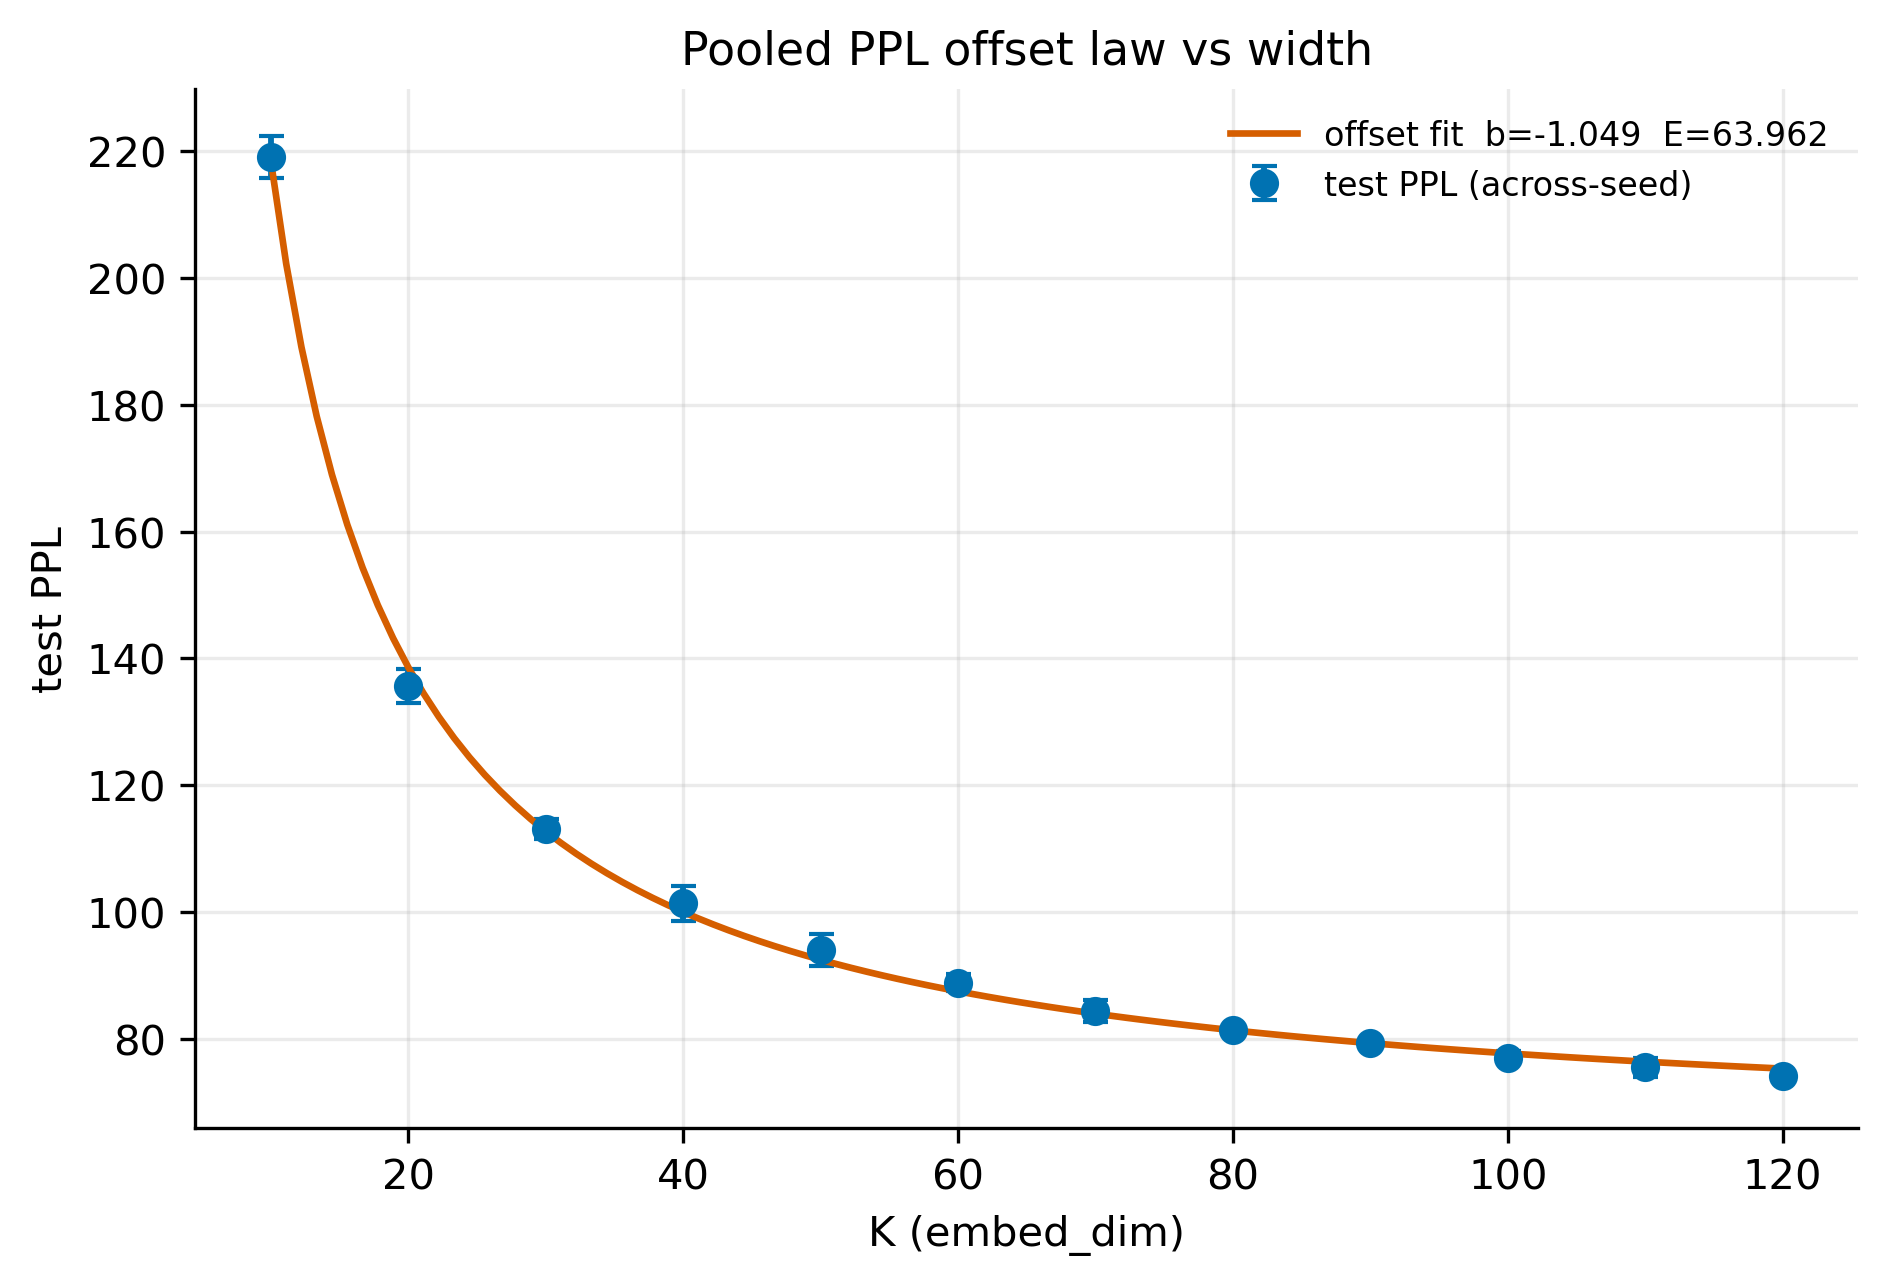
\includegraphics[width=0.72\linewidth]{attention/figs/vfe3_gl10_ppl_vs_embed_dim_offset.png}
\caption{Mean test perplexity versus embedding dimension for the fixed-$\mathrm{GL}^+(10)$ development-provenance sweep, with the descriptive offset fit over the observed width range.}
\label{fig:vfe3_gl10_scaling}
\end{figure}

\subsection{Divergence Order}
The current release has no matching test-result and provenance package for the historical single-seed divergence-order comparison. Its numerical results are unsupported-current and are omitted; the comparison cannot presently be treated as empirical evidence for selecting the forward KL.

\subsection{Positional-Prior Extrapolation}
The current release likewise has no matching test-result and provenance package for the historical single-seed positional-prior comparison. Its numerical results and ranking claims are unsupported-current and are omitted.


% bibliographystyle is set by jmlr2e
\bibliography{references}

\end{document}
